\documentclass[gmd,manuscript,online]{copernicus}
%DIF LATEXDIFF DIFFERENCE FILE
%DIF DEL main_v0.tex   Fri Sep 20 13:33:44 2024
%DIF ADD main_v1.tex   Fri Sep 20 16:53:57 2024

% ============================================================
% packages: base packages and hardly taggable stuff
% ============================================================
\usepackage[utf8]{inputenc}
\usepackage[T1]{fontenc}
\usepackage{newunicodechar}
\usepackage{lmodern}
\usepackage{anyfontsize}
\usepackage{enumitem}  % in conflict with \usepackage{enumerate}
%\usepackage{fourier}  % style
%\usepackage{lipsum}  % dummy text
%\usepackage{authblk}  % footnote style author/affiliation
%\usepackage[top=2cm, bottom=3cm, left=2cm, right=2cm, scale=0.75]{geometry}  % set the margins
%\usepackage[inner=3cm, textwidth=445pt, scale=0.75, top=3cm, bottom=3cm]{geometry}  % set the margins (book style)
\usepackage{fancyvrb}  % insert verbatim within a command
\usepackage{fancyhdr}  % set header and footer
\usepackage[letterspace=150]{microtype}  % improved typographics
\usepackage{textcomp}  % more text symbols
% \usepackage{gensymb}  % more text and math symbols - clash!!!
\usepackage{bbm}  % blackboard-style cm fonts
\usepackage{csvsimple}  % csv file processing
\usepackage[bottom]{footmisc}  % footnotes at the bottom of the page
\usepackage{stackengine}  % stack objects vertically in a variety of customizable ways
\usepackage{ragged2e}  % \justify

% new page
\newcommand{\NewPage}{\newpage\null\thispagestyle{empty}\newpage}

% no indent
%\setlength\parindent{0pt}

% ============================================================
% packages: math
% ============================================================
\usepackage{bm}  % access bold symbols in math mode
\usepackage{amsmath,etoolbox}
\allowdisplaybreaks
\usepackage{amsfonts}
\usepackage{amstext}
\usepackage{amssymb}
\usepackage{amsthm}
\usepackage{empheq}
\usepackage{cases}
\usepackage{mathtools}
\usepackage{nicefrac}  % diagonal fractions

% ============================================================
% math aliases and commands
% ============================================================
% enumerate subequations with arabic numbers (e.g. 1.1, 1.2, ecc)
\patchcmd{\subequations}{\def\theequation{\theparentequation\alph{equation}}}{\def\theequation{\theparentequation.\arabic{equation}}}{}{}

%\usepackage{chngcntr}
%\counterwithout{equation}{section} % undo numbering system provided by phstyle.cls
%\counterwithin{equation}{chapter}  % implement desired numbering system

% absolute value
\DeclarePairedDelimiter\abs{\lvert}{\rvert}
\makeatletter
\let\oldabs\abs
\def\abs{\@ifstar{\oldabs}{\oldabs*}}

% argmin
\DeclareMathOperator*{\argmin}{arg\,min}

% norm symbol
\newcommand{\norm}[1]{\left\lVert#1\right\rVert}

% mod symbol
\newcommand{\Mod}[1]{\ (\mathrm{mod}\ #1)}

% aliases for \widetilde
\newcommand{\wt}[1]{\widetilde{#1}}

% make \big| adapt to the context
\makeatletter
\let\amstexbig\big
\def\newbig#1{%
	\ifx#1|%
	\expandafter\@firstoftwo
	\else
		\expandafter\@secondoftwo
	\fi
		{\big@bar}%
		{\amstexbig{#1}}%
}
\AtBeginDocument{\let\big\newbig}
\def\big@bar{\bBigg@{1.1}|}
\makeatother

% theorem and definition environment
\theoremstyle{theorem}
\newtheorem{theorem}{Theorem}[section]
\theoremstyle{definition}
\newtheorem{definition}{Definition}[section]
\theoremstyle{remark}
\newtheorem{remark}{Remark}[section]
\theoremstyle{proposition}
\newtheorem{proposition}{Proposition}[section]
%\newenvironment{definition}[1][Definition]{\begin{trivlist}
%\item[\hskip \labelsep {\bfseries #1}]}{\end{trivlist}}

% enumerate the equations and the figures according to the section they are in
%\numberwithin{equation}{section}
%\numberwithin{figure}{chapter}

% inline fractions settings
\renewcommand{\textfraction}{0.1}
\renewcommand{\topfraction}{0.9}

% matrices
%DIF 114c114
%DIF < %\newcommand{\matr}[1]{\mathbf{#1}}  % undergraduate algebra version
%DIF -------
\newcommand{\matr}[1]{\mathbf{#1}}  % undergraduate algebra version %DIF > 
%DIF -------
%\newcommand{\matr}[1]{#1}          % pure math version
%\newcommand{\matr}[1]{\bm{#1}}     % ISO complying version

% interrupting and resuming subequations
\makeatletter
\newcounter{qrr@oldeq}
\newcounter{qrr@oldsubeq}
\newcounter{qrr@realeq}
\renewenvironment{subequations}{%
	\refstepcounter{equation}%
	\protected@edef\theparentequation{\theequation}%
	\setcounter{parentequation}{\value{equation}}%
	\setcounter{equation}{0}%
	\def\theequation{\theparentequation\alph{equation}}%
	\ignorespaces
	}{%
	\setcounter{qrr@oldeq}{\value{parentequation}}%
	\setcounter{qrr@oldsubeq}{\value{equation}}%
	\setcounter{equation}{\value{parentequation}}%
	\ignorespacesafterend
}
\newenvironment{subequations*}{%
	\setcounter{qrr@realeq}{\value{equation}}%
	\let\theparentequation\theequation%
	\patchcmd{\theparentequation}{equation}{parentequation}{}{}%
	\setcounter{parentequation}{\numexpr\value{qrr@oldeq}-1}%
	\setcounter{equation}{\value{qrr@oldsubeq}}%
	\def\theequation{\theparentequation\alph{equation}}%
	\refstepcounter{parentequation}%
	\ignorespaces
	}{%
	\setcounter{qrr@oldeq}{\value{parentequation}}%
	\setcounter{qrr@oldsubeq}{\value{equation}}%
	\setcounter{equation}{\value{qrr@realeq}}%
	\ignorespacesafterend
}
\makeatother

% aliases for greek letters
\newcommand{\bchi}{\bm{\chi}}
\newcommand{\bphi}{\bm{\phi}}
\newcommand{\bpsi}{\bm{\psi}}
\newcommand{\bxi}{\bm{\xi}}

% imaginary unit
\newcommand{\iu}{\text{i}}

% math environments patched to enable proper line numbering
% \newenvironment{myeq}{\begin{linenomath*}\begin{equation}}{\end{equation}\end{linenomath*}}
% \newenvironment{myeq*}{\begin{linenomath*}\begin{equation*}}{\end{equation*}\end{linenomath*}}
% \newenvironment{myalign}{\begin{linenomath*}\begin{align}}{\end{align}\end{linenomath*}}
% \newenvironment{myalign*}{\begin{linenomath*}\begin{align*}}{\end{align*}\end{linenomath*}}

% ============================================================
% packages: tabular
% ============================================================
\usepackage{longtable}
\usepackage{tabu}
\usepackage{multicol}
\usepackage{multirow}
\usepackage{array}
\usepackage{makecell}
\usepackage{booktabs}
\usepackage{hhline}

% ============================================================
% packages: hyperlinks
% ============================================================
% \RequirePackage[hyphens]{url}
% \PassOptionsToPackage{hyphens}{url}\usepackage{hyperref}
\usepackage{breakurl}
\usepackage{url}

% ============================================================
% packages: graphics
% ============================================================
%\usepackage{floatrow}	% notes below a figure
\usepackage{pdfpages}  % include pdf documents
\usepackage{graphicx}
\usepackage{epstopdf}
%\epstopdfsetup{outdir=/Users/subbiali/Desktop/phd/manuscripts/pdc_paper/img/epstopdf/}
\usepackage{float}
\usepackage[position = top]{subfig}
\usepackage{wrapfig}
\usepackage[labelfont=bf,labelsep=period,font=small]{caption}
% \usepackage{subcaption}  % in conflict with \usepackage{subfloat}
\usepackage{tikz}
\usetikzlibrary{decorations.pathreplacing}

% modify the space between figure and caption
%\setlength{\abovecaptionskip}{-4pt}
%\setlength{\belowcaptionskip}{3pt}

% ============================================================
% packages: pseudocode
% ============================================================
%DIF 211c211
%DIF < %\usepackage{algorithm}
%DIF -------
\usepackage{algorithm} %DIF > 
%DIF -------
\usepackage[noend]{algpseudocode}

% fancy "for" block
%DIF 215-217c215-217
%DIF < %\algnewcommand\algorithmicto{\textbf{to}}
%DIF < %\algrenewtext{For}[3]%
%DIF < %{\algorithmicfor\ $#1 \gets #2$ \algorithmicto\ $#3$ \algorithmicdo}
%DIF -------
\algnewcommand\algorithmicto{\textbf{to}} %DIF > 
\algrenewtext{For}[3]% %DIF > 
{\algorithmicfor\ $#1 \gets #2$ \algorithmicto\ $#3$ \algorithmicdo} %DIF > 
%DIF -------

% redefine \Require and \Ensure for algorithm environment
%\renewcommand{\algorithmicrequire}{\textbf{Input:}}
%\renewcommand{\algorithmicensure}{\textbf{Output:}}

% define the do-while loop
%\algdef{SE}[DOWHILE]{DoWhile}{EndDoWhile}{\algorithmicdo}[1]{\algorithmicwhile\ #1}

% ============================================================
% packages: fancy boxes
% ============================================================
\usepackage[export]{adjustbox}

\usepackage[many]{tcolorbox}
%\makeatletter
%	\renewcommand*\l@figure{\@dottedtocline{1}{1em}{3.2em}}
%\makeatother

% ============================================================
% packages: listings
% ============================================================
\usepackage{listings}

% minted: package for formatting and highlighting source code
\usepackage[cache=true]{minted}
\usemintedstyle{default}
\setminted{mathescape, escapeinside=||, tabsize=4, fontfamily=tt}
\newmint[py]{python}{python3=true}
\newmintinline[pyinline]{python}{python3=true}

% ============================================================
% packages: bibliography
% ============================================================
% \usepackage[authoryear, round, sort, nonamebreak]{natbib}
\bibliographystyle{copernicus}

% ============================================================
% graphics path
% ============================================================
\graphicspath{{./../../img}}

% ============================================================
% packages: template specific
% ============================================================
\usepackage{lineno}
% \usepackage[inline]{trackchanges} %for better track changes. finalnew option will compile document with changes incorporated.
\usepackage{soul}
\linenumbers

%DIF 267a267-271
% ============================================================ %DIF > 
% subfiles %DIF > 
% ============================================================ %DIF > 
\usepackage{subfiles} %DIF > 
 %DIF > 
%DIF -------
% allow \cite in subfiles
\makeatletter
\patchcmd{\nocite}{\ifx\@onlypreamble\document}{\iftrue}{}{}
\makeatother

% make references pop-up in subfiles
% note: this does not seem to work...
%DIF 274c279
%DIF < %\def\biblio{\bibliography{references}}
%DIF -------
\def\biblio{\bibliography{references}} %DIF > 
%DIF -------

% ============================================================
% line spacing
% ============================================================
\usepackage{setspace}
%\doublespacing
%DIF 281-286d286
%DIF < 
%DIF < % ============================================================
%DIF < % subfiles
%DIF < % ============================================================
%DIF < \usepackage{subfiles}
%DIF < 
%DIF -------

% ============================================================
% begin document
% ============================================================
%DIF PREAMBLE EXTENSION ADDED BY LATEXDIFF
%DIF UNDERLINE PREAMBLE %DIF PREAMBLE
\RequirePackage[normalem]{ulem} %DIF PREAMBLE
\RequirePackage{color}\definecolor{RED}{rgb}{1,0,0}\definecolor{BLUE}{rgb}{0,0,1} %DIF PREAMBLE
\providecommand{\DIFadd}[1]{{\protect\color{blue}\uwave{#1}}} %DIF PREAMBLE
\providecommand{\DIFdel}[1]{{\protect\color{red}\sout{#1}}} %DIF PREAMBLE
%DIF SAFE PREAMBLE %DIF PREAMBLE
\providecommand{\DIFaddbegin}{} %DIF PREAMBLE
\providecommand{\DIFaddend}{} %DIF PREAMBLE
\providecommand{\DIFdelbegin}{} %DIF PREAMBLE
\providecommand{\DIFdelend}{} %DIF PREAMBLE
\providecommand{\DIFmodbegin}{} %DIF PREAMBLE
\providecommand{\DIFmodend}{} %DIF PREAMBLE
%DIF FLOATSAFE PREAMBLE %DIF PREAMBLE
\providecommand{\DIFaddFL}[1]{\DIFadd{#1}} %DIF PREAMBLE
\providecommand{\DIFdelFL}[1]{\DIFdel{#1}} %DIF PREAMBLE
\providecommand{\DIFaddbeginFL}{} %DIF PREAMBLE
\providecommand{\DIFaddendFL}{} %DIF PREAMBLE
\providecommand{\DIFdelbeginFL}{} %DIF PREAMBLE
\providecommand{\DIFdelendFL}{} %DIF PREAMBLE
\newcommand{\DIFscaledelfig}{0.5}
%DIF HIGHLIGHTGRAPHICS PREAMBLE %DIF PREAMBLE
\RequirePackage{settobox} %DIF PREAMBLE
\RequirePackage{letltxmacro} %DIF PREAMBLE
\newsavebox{\DIFdelgraphicsbox} %DIF PREAMBLE
\newlength{\DIFdelgraphicswidth} %DIF PREAMBLE
\newlength{\DIFdelgraphicsheight} %DIF PREAMBLE
% store original definition of \includegraphics %DIF PREAMBLE
\LetLtxMacro{\DIFOincludegraphics}{\includegraphics} %DIF PREAMBLE
\newcommand{\DIFaddincludegraphics}[2][]{{\color{blue}\fbox{\DIFOincludegraphics[#1]{#2}}}} %DIF PREAMBLE
\newcommand{\DIFdelincludegraphics}[2][]{% %DIF PREAMBLE
\sbox{\DIFdelgraphicsbox}{\DIFOincludegraphics[#1]{#2}}% %DIF PREAMBLE
\settoboxwidth{\DIFdelgraphicswidth}{\DIFdelgraphicsbox} %DIF PREAMBLE
\settoboxtotalheight{\DIFdelgraphicsheight}{\DIFdelgraphicsbox} %DIF PREAMBLE
\scalebox{\DIFscaledelfig}{% %DIF PREAMBLE
\parbox[b]{\DIFdelgraphicswidth}{\usebox{\DIFdelgraphicsbox}\\[-\baselineskip] \rule{\DIFdelgraphicswidth}{0em}}\llap{\resizebox{\DIFdelgraphicswidth}{\DIFdelgraphicsheight}{% %DIF PREAMBLE
\setlength{\unitlength}{\DIFdelgraphicswidth}% %DIF PREAMBLE
\begin{picture}(1,1)% %DIF PREAMBLE
\thicklines\linethickness{2pt} %DIF PREAMBLE
{\color[rgb]{1,0,0}\put(0,0){\framebox(1,1){}}}% %DIF PREAMBLE
{\color[rgb]{1,0,0}\put(0,0){\line( 1,1){1}}}% %DIF PREAMBLE
{\color[rgb]{1,0,0}\put(0,1){\line(1,-1){1}}}% %DIF PREAMBLE
\end{picture}% %DIF PREAMBLE
}\hspace*{3pt}}} %DIF PREAMBLE
} %DIF PREAMBLE
\LetLtxMacro{\DIFOaddbegin}{\DIFaddbegin} %DIF PREAMBLE
\LetLtxMacro{\DIFOaddend}{\DIFaddend} %DIF PREAMBLE
\LetLtxMacro{\DIFOdelbegin}{\DIFdelbegin} %DIF PREAMBLE
\LetLtxMacro{\DIFOdelend}{\DIFdelend} %DIF PREAMBLE
\DeclareRobustCommand{\DIFaddbegin}{\DIFOaddbegin \let\includegraphics\DIFaddincludegraphics} %DIF PREAMBLE
\DeclareRobustCommand{\DIFaddend}{\DIFOaddend \let\includegraphics\DIFOincludegraphics} %DIF PREAMBLE
\DeclareRobustCommand{\DIFdelbegin}{\DIFOdelbegin \let\includegraphics\DIFdelincludegraphics} %DIF PREAMBLE
\DeclareRobustCommand{\DIFdelend}{\DIFOaddend \let\includegraphics\DIFOincludegraphics} %DIF PREAMBLE
\LetLtxMacro{\DIFOaddbeginFL}{\DIFaddbeginFL} %DIF PREAMBLE
\LetLtxMacro{\DIFOaddendFL}{\DIFaddendFL} %DIF PREAMBLE
\LetLtxMacro{\DIFOdelbeginFL}{\DIFdelbeginFL} %DIF PREAMBLE
\LetLtxMacro{\DIFOdelendFL}{\DIFdelendFL} %DIF PREAMBLE
\DeclareRobustCommand{\DIFaddbeginFL}{\DIFOaddbeginFL \let\includegraphics\DIFaddincludegraphics} %DIF PREAMBLE
\DeclareRobustCommand{\DIFaddendFL}{\DIFOaddendFL \let\includegraphics\DIFOincludegraphics} %DIF PREAMBLE
\DeclareRobustCommand{\DIFdelbeginFL}{\DIFOdelbeginFL \let\includegraphics\DIFdelincludegraphics} %DIF PREAMBLE
\DeclareRobustCommand{\DIFdelendFL}{\DIFOaddendFL \let\includegraphics\DIFOincludegraphics} %DIF PREAMBLE
%DIF AMSMATHULEM PREAMBLE %DIF PREAMBLE
\makeatletter %DIF PREAMBLE
\let\sout@orig\sout %DIF PREAMBLE
\renewcommand{\sout}[1]{\ifmmode\text{\sout@orig{\ensuremath{#1}}}\else\sout@orig{#1}\fi} %DIF PREAMBLE
\makeatother %DIF PREAMBLE
%DIF COLORLISTINGS PREAMBLE %DIF PREAMBLE
\RequirePackage{listings} %DIF PREAMBLE
\RequirePackage{color} %DIF PREAMBLE
\lstdefinelanguage{DIFcode}{ %DIF PREAMBLE
%DIF DIFCODE_UNDERLINE %DIF PREAMBLE
  moredelim=[il][\color{red}\sout]{\%DIF\ <\ }, %DIF PREAMBLE
  moredelim=[il][\color{blue}\uwave]{\%DIF\ >\ } %DIF PREAMBLE
} %DIF PREAMBLE
\lstdefinestyle{DIFverbatimstyle}{ %DIF PREAMBLE
	language=DIFcode, %DIF PREAMBLE
	basicstyle=\ttfamily, %DIF PREAMBLE
	columns=fullflexible, %DIF PREAMBLE
	keepspaces=true %DIF PREAMBLE
} %DIF PREAMBLE
\lstnewenvironment{DIFverbatim}{\lstset{style=DIFverbatimstyle}}{} %DIF PREAMBLE
\lstnewenvironment{DIFverbatim*}{\lstset{style=DIFverbatimstyle,showspaces=true}}{} %DIF PREAMBLE
\lstset{extendedchars=\true,inputencoding=utf8}

%DIF END PREAMBLE EXTENSION ADDED BY LATEXDIFF

\begin{document}
	\justify

	% ============================================================
	% title, authors and affiliations
	% ============================================================
	\title{Exploring a high-level programming model for the NWP domain using ECMWF microphysics schemes}

	% \Author[affil]{given_name}{surname}
	\Author[1]{Stefano}{Ubbiali}
	\Author[2]{Christian}{K\"uhnlein}
	\Author[1]{Christoph}{Sch\"ar}
	\Author[3]{Linda}{Schlemmer}
	\Author[4,5]{Thomas C.}{Schulthess}
	\Author[2]{Michael}{Staneker}
	\Author[1]{Heini}{Wernli}

	% \affil[]{ADDRESS}
	\affil[1]{Institute for Atmospheric and Climate Science (IAC), ETH Z\"urich, Switzerland}
	\vspace*{0.1cm}
	\affil[2]{European Centre for Medium-Range Weather Forecasts (ECMWF), Bonn, Germany}
	\vspace*{0.1cm}
	\affil[3]{Deutscher Wetterdienst (DWD), Offenbach, Germany}
	\vspace*{0.1cm}
	\affil[4]{Institute for Theoretical Physics (ITP), ETH Z\"urich, Switzerland}
	\vspace*{0.1cm}
	\affil[5]{Swiss National Supercomputing Centre (CSCS), Lugano, Switzerland}

	\correspondence{Stefano Ubbiali (subbiali@phys.ethz.ch)}

	\runningtitle{Exploring a high-level programming model for the NWP domain using ECMWF microphysics schemes}

	\runningauthor{S. Ubbiali et al.}

	%% These dates will be inserted by Copernicus Publications during the typesetting process.
	\received{}
	\pubdiscuss{} %% only important for two-stage journals
	\revised{}
	\accepted{}
	\published{}

	\firstpage{1}

	\maketitle

	\doublespacing

	% ============================================================
	% abstract
	% ============================================================
	\begin{abstract}
		We explore the domain-specific Python library GT4Py (GridTools for Python) for implementing a representative physical parametrization scheme and the related tangent-linear \& adjoint algorithms from the Integrated Forecasting System (IFS) of ECMWF. GT4Py encodes stencil operators in an abstract and hardware-agnostic fashion, thus enabling more concise, readable and maintainable scientific applications. The library achieves high performance by translating the application into targeted low-level coding implementations. Here, the main goal is to study the correctness and performance-portability of the Python rewrites with GT4Py against the reference Fortran code and a number of automatically and manually ported variants created by ECMWF. The present work is part of a larger cross-institutional effort to port weather and climate models to Python with GT4Py. The focus of the current work is the IFS prognostic cloud microphysics scheme, a core physical parametrization represented by a comprehensive code that takes a significant share of the total forecast model execution time. In order to verify GT4Py for Numerical Weather Prediction (NWP) systems, we put additional emphasis on the implementation and validation of the tangent-linear and adjoint model versions which are employed in data assimilation. We benchmark all prototype codes on three European supercomputers characterized by diverse GPU and CPU hardware, node designs, software stacks and compiler suites. Once the application is ported to Python with GT4Py, we find excellent portability, competitive \DIFaddbegin \DIFadd{GPU }\DIFaddend performance, and robust execution in all tested scenarios including with \DIFdelbegin \DIFdel{reduced }\DIFdelend \DIFaddbegin \DIFadd{single }\DIFaddend precision.
	\end{abstract}

	% ============================================================
	% section 1
	% ============================================================
	\section{Introduction}
	\label{section:introduction}

	Soon after its first public release in 1957, Fortran \DIFdelbegin \DIFdel{has become }\DIFdelend \DIFaddbegin \DIFadd{became }\DIFaddend the language of choice for weather and climate models \citep{mendez14}. On the one hand, its \DIFdelbegin \DIFdel{functional }\DIFdelend \DIFaddbegin \DIFadd{procedural }\DIFaddend programming style and built-in support for multi-dimensional arrays has granted Fortran large popularity in the whole scientific computing community. On the other, its low-level nature guarantees fast execution of intensive mathematical operations on vector machines and conventional Central Processing Units (CPUs). In the last decades, these characteristics have permitted to run weather forecasts several times per day under tight operational schedules on High-Performance Computing (HPC) systems \citep{neumann19}.

	In recent years, in response to the simultaneous end of Moore's law and Dennard scaling, and due to the societal challenge to reduce energy consumption, the computer hardware landscape has been undergoing a rapid specialization to prevent unsustainable growth of the power envelope \citep{muller19}. As a result, most supercomputers nowadays have a heterogeneous node design, where energy-efficient accelerators such as Graphics Processing Units (GPUs) co-exist with traditional CPUs. Because Fortran has been conceived with CPU-centric machines in mind, efficient programming of hybrid HPC platforms using the core Fortran language can be challenging \citep{mendez14, lawrence18}. Indeed, the sustained performance of legacy weather and climate model codes written in Fortran has decreased over the decades \citep{schulthess18}, revealing the urgency for algorithmic and software adaptations to remain competitive in the medium and long term \citep{bauer21}.

	Compiler directives (or pragmas) are an attractive solution for parallelization, both to spread a workload across multiple CPU threads, and to offload data and computations to GPU. The most famous incarnations of this programming paradigm are OpenMP \citep{dagum98} and OpenACC \citep{chandrasekaran17}. Because compiler directives accommodate incremental porting and enable non-disruptive software development workflows, they are adopted by many weather and climate modeling groups, who are facing the grand challenge of accelerating large code-bases with thousands of source files and millions of lines of code, which stem from decades of scientific discoveries and software developments \citep{lapillonne17, lapillonne20, randall22}. In order not to threaten the overall readability of the code by exposing low-level instructions, the annotation of Fortran codes with compiler directives can be automated in the pre-processor step of the compilation process using tools such as the CLAW compiler \citep{clement19} or the ECMWF source-to-source translation tool Loki\footnote{\url{github.com/ecmwf-ifs/loki}}. Although pragma-based programming models can support intrusive hardware-specific code transformations, additional specialized optimizations may still be required, which could finally lead to code duplication and worsen maintainability \citep{dahm23}. Moreover, performance and portability are much dependent on the level of support and optimization offered by the compiler stack.

	On the contrary, domain-specific languages (DSLs) separate the code describing the science from the code actually executing on the target hardware, thus enabling \emph{performance-portability}, namely application codes that achieve near-optimal performance on a variety of computer architectures \citep{deakin19}. Large portions of many modeling systems are being rewritten using multiple and diverse DSLs, not necessarily embedded in Fortran. For instance, the dynamical core of the weather prediction model from the COnsortium for Small-scale MOdeling \citep[COSMO;][]{baldauf11} has been rewritten in C++ using the GridTools library \citep{afanasyev21} to port stencil-based operators to GPUs \citep{fuhrer14, fuhrer18}. Similarly, HOMMEXX-NH \citep{bertagna20} is an architecture-portable C++ implementation of the non-hydrostatic dynamical core of the Energy Exascale Earth System model \citep[E3SM;][]{taylor20} harnessing the Kokkos library to express on-node parallelism \citep{edwards14}. The GungHo project for a new dynamical core at the UK Met Office \DIFaddbegin \DIFadd{\mbox{%DIFAUXCMD
\citep{melvin19, melvin24} }\hskip0pt%DIFAUXCMD
}\DIFaddend blends the LFRic infrastructure with the PSyclone code generator \citep{adams19}. Pace \citep{ben-nun22, dahm23} is a Python rewrite of the Finite-Volume Cubed-Sphere Dynamical Core \citep[FV3;][]{harris13} using GT4Py to accomplish performance-portability and productivity. Similarly, various Swiss partners including MeteoSwiss, ETH Zurich and CSCS are porting the ICOsahedral Non-hydrostatic modeling framework \citep[ICON;][]{zangl15} to GT4Py \citep{luz24}. In another related project \citep{kuhnlein23}, a next-generation model for the IFS at ECMWF is developed in Python with GT4Py building on FVM \citep{smolarkiewicz16, kuehnlein19}.

	The focus of the portability efforts mentioned above is the model dynamical core - the part of the model solving numerically the fundamental nonlinear fluid-dynamics equations. In the present work, we turn the attention to physical parametrizations - which account for the representation of subgrid-scale processes - and additionally address the associated tangent-linear and adjoint algorithms. Parametrizations are being commonly ported to accelerators using OpenACC \citep[e.g., ][]{fuhrer14, yang19, kim21}. Wrappers around low-level legacy physics codes might then be designed to facilitate adoption within higher-level workflows \citep{monteiro18, mcgibbon21}. Lately, first attempts at refactoring physical parametrizations with respect to portability have been documented in the literature. For instance, \citet{watkins23} presented a rewrite of the MPAS-Albany Land Ice (MALI) ice-sheet model using Kokkos. Here, we present a Python implementation of the cloud microphysics schemes CLOUDSC \DIFaddbegin \DIFadd{\mbox{%DIFAUXCMD
\citep{gt4py-dwarf-p-cloudsc} }\hskip0pt%DIFAUXCMD
}\DIFaddend and CLOUDSC2 \DIFaddbegin \DIFadd{\mbox{%DIFAUXCMD
\citep{gt4py-dwarf-p-cloudsc2-tl-ad}}\hskip0pt%DIFAUXCMD
}\DIFaddend , which are part of the physics suite of the IFS at ECMWF\footnote{As we mention in Section \ref{section:target-cloud-microphysics-schemes}, the versions of CLOUDSC and CLOUDSC2 considered in this study correspond to older release cycles of the IFS than the one currently used in production.}. Details on the formulation and validation of the schemes are discussed in Section \ref{section:target-cloud-microphysics-schemes}. The proposed Python implementations build upon the GT4Py toolchain, and in the remainder of the paper we use the term CLOUDSC-GT4Py to refer to the GT4Py rewrite of CLOUDSC, while the GT4Py ports of the nonlinear, tangent-linear and adjoint formulations of CLOUDSC2 are collectively referred to as CLOUDSC2-GT4Py. The working principles of the GT4Py framework are illustrated in Section \ref{section:domain-specific-approach-to-scientific-software-development}, where we also advocate the advantages offered by domain-specific software approaches. Section \ref{section:infrastructure-code} sheds some light on the infrastructure code \DIFaddbegin \DIFadd{\mbox{%DIFAUXCMD
\citep{ifs-physics-common}}\hskip0pt%DIFAUXCMD
}\DIFaddend , and how it can enable composable and reusable model components. In Section \ref{section:performance-analysis}, we compare the performance of CLOUDSC-GT4Py and CLOUDSC2-GT4Py, as measured on three leadership-class GPU-equipped supercomputers, to established implementations in Fortran and C/C++. We conclude the paper with final remarks and future development paths.

	% ============================================================
	% section 2
	% ============================================================
	\section{Defining the targeted scientific applications}
	\label{section:target-cloud-microphysics-schemes}

	Several physical and chemical mechanisms occurring in the atmosphere are active on spatial scales that are significantly smaller than the highest affordable model resolution. It follows that these mechanisms cannot be properly captured by the resolved model dynamics, but need to be \emph{parametrized}. Parametrizations express the bulk effect of subgrid-scale phenomena on the resolved flow in terms of the grid-scale variables. The equations underneath physical parametrizations are based on theoretical and semi-empirical arguments, and their numerical treatment commonly adheres to the \emph{single-column} abstraction, so that adjustments can only happen within individual columns, with no data dependencies between columns. The atmospheric module of the IFS includes parametrizations dealing with the radiative heat transfer, deep and shallow convection, clouds and stratiform precipitation, surface exchange, turbulent mixing in the planetary boundary layer, subgrid-scale orographic drag, non-orographic gravity wave drag, and methane oxidation \citep{ifs48r1}.

	The focus of this paper is on the cloud microphysics modules of the ECMWF: the CLOUDSC -- used in operational forecasting -- and the CLOUDSC2 -- employed in the data assimilation. The motivation is three-fold: (i) both schemes are among the most computationally expensive parametrizations, with the CLOUDSC accounting for up to $10\%$ of the total execution time of the high-resolution operational forecasts at ECMWF; (ii) they are representative of the computational patterns ubiquitous in physical parametrizations; and (iii) they already exist in the form of \emph{dwarfs}. The weather and climate ``computational dwarfs'', or simply ``dwarfs'', are model components shaped into stand-alone software packages to serve as archetypes of relevant computational motifs \citep{muller19} and provide a convenient platform for performance optimizations and portability studies \citep{bauer20}. In recent years, the Performance and Portability Team of ECMWF created the CLOUDSC and CLOUDSC2 dwarfs. The original Fortran codes for both packages, corresponding respectively to the IFS Cycle 41r2 and 46r1, have been pulled out of the IFS codebase, slightly polished\DIFaddbegin \footnote{\DIFadd{Compared to the original implementations run operationally at ECMWF, the CLOUDSC \& CLOUDSC2 dwarf codes do not include (i) all the IFS-specific infrastructure code, (ii) the calculation of budget diagnostics, and (iii) dead code paths.}} \DIFaddend and finally made available in public code repositories\footnote{\url{https://github.com/ecmwf-ifs/dwarf-p-cloudsc} and \url{https://github.com/ecmwf-ifs/dwarf-p-cloudsc2-tl-ad}}. Later, the repositories have been enriched with alternative coding implementations, using different languages and programming paradigms; the most relevant implementations will be discussed in Section \ref{section:performance-analysis}.

	\subsection{CLOUDSC: Cloud microphysics of the forecast model}

	The CLOUDSC is a single-moment cloud microphysics scheme that parametrizes stratiform clouds and their contribution to surface precipitation \citep{ifs48r1}. It was implemented in the IFS Cycle 36r4 and has been operational at ECMWF since November 2010. Compared to the pre-existing scheme, it accounts for five prognostic variables (cloud fraction, cloud liquid water, cloud ice, rain and snow) and brings substantial enhancements in different aspects, including treatment of mixed-phase clouds, advection of precipitating hydrometeors (rain and snow), physical realism, and numerical stability \citep{nogherotto16}. For a comprehensive description of the scheme, we refer the reader to \citet{forbes11b} and the references therein. For all the coding versions considered in this paper, including the novel Python rewrite, the calculations are validated by direct comparison of the output against serialized language-agnostic reference data provided by ECMWF.

	\subsection{CLOUDSC2: Cloud microphysics in the context of data assimilation}
	\DIFaddbegin \label{section:cloudsc2}
\DIFaddend 

	The CLOUDSC2 scheme represents a streamlined version of CLOUDSC, devised for use in the four-dimensional variational assimilation (4D-Var) at ECMWF \citep{courtier94}. 4D-Var merges short-term model integrations with observations over a twelve-hour assimilation window to determine the best possible representation of the current state of the atmosphere. This then provides the initial conditions for longer-term forecasts \citep{janiskova23}. The optimal synthesis between model and observational data is found by minimizing a cost function, which is evaluated using the \emph{tangent-linear} of the \emph{non-linear} forecasting model, while the \emph{adjoint} model is employed to compute the gradient of the cost function \citep{errico97, janiskova99}. For the sake of computational economy, the tangent-linear and adjoint operators are derived from a simplified and regularized version of the full non-linear model. The CLOUDSC2 is one of the physical parametrizations included in the ECMWF's simplified model, together with radiation, vertical diffusion, orographic wave drag, moist convection, and non-orographic gravity wave activity \citep{janiskova23}. In the following, we provide a mathematical and algorithmic representation of the tangent-linear and adjoint versions of CLOUDSC2. For the sake of brevity, in the rest of the paper we will refer to the non-linear, tangent-linear and adjoint formulations of CLOUDSC2 using CLOUDSC2NL, CLOUDSC2TL and CLOUDSC2AD, respectively.

	\DIFdelbegin %DIFDELCMD < \begin{algorithm}[t!]
%DIFDELCMD < 		%%%
%DIFDELCMD < \caption{%
{%DIFAUXCMD
\DIFdel{The Taylor test assessing the formal correctness of the coding implementation of the tangent-linear formulation of CLOUDSC2, denoted as }\textsc{\DIFdel{CLOUDSC2TL}}%DIFAUXCMD
\DIFdel{. The three-dimensional arrays $\mathbf{x}$ and $\mathbf{y}$ collect the grid point values for all $nin$ input fields and $nout$ output fields of CLOUDSC2, respectively. The corresponding variations are $\delta \mathbf{x}$ and $\delta \mathbf{y}$. The grid consists of $ncol$ columns, each containing $nlev$ vertical levels. Note that compared to its functional counterpart $F' \left[\boldsymbol{x} \right] : \delta \boldsymbol{x} \mapsto \delta \boldsymbol{y}$, }\textsc{\DIFdel{CLOUDSC2TL($\mathbf{x}, \, \delta \mathbf{x}$)}} %DIFAUXCMD
\DIFdel{returns both $\mathbf{y}$ and $\delta \mathbf{y}$. The coding implementation of the non-linear CLOUDSC2 is indicated as }\textsc{\DIFdel{CLOUDSC2NL}}%DIFAUXCMD
\DIFdel{.}}
		%DIFAUXCMD
%DIFDELCMD < \label{alg:taylor-test}
%DIFDELCMD < 

%DIFDELCMD < 		\begin{algorithmic}[1]
%DIFDELCMD < 			%%%
%DIF <  \Function{GetFieldSum}{$ncol, \, nlev, \, \boldsymbol{f}$} \Comment{$\boldsymbol{f} \in \mathbb{R}^{ncol \times nlev}$}
			%DIF <      \State $field\_sum ~ \gets ~ 0$
			%DIF <      \For{i}{1}{ncol}
			%DIF <          \For{k}{1}{nlev}
			%DIF <              \State $field\_sum \gets sum + \boldsymbol{f}(i, \, k)$
			%DIF <          \EndFor
			%DIF <      \EndFor
			%DIF <      \State \textbf{return} $field\_sum$
			%DIF <  \EndFunction
%DIFDELCMD < 

%DIFDELCMD < 			%%%
%DIF <  \Statex
%DIFDELCMD < 

%DIFDELCMD < 			\Function{TotalNorm}{$ncol, \, nlev, \, nout, \, \mathbf{y}, \, \mathbf{y}_j, \, \delta \mathbf{y}_j$} \Comment{$\mathbf{y}, \, \mathbf{y}_j, \, \delta \mathbf{y}_j \in \mathbb{R}^{ncol \times nlev \times nout}$}
%DIFDELCMD < 			\State %%%
\DIFdel{$total\_norm ~ \gets ~ 0$
			}%DIFDELCMD < \State %%%
\DIFdel{$total\_count ~ \gets ~ 0$
			}%DIFDELCMD < \For{l}{1}{nout}
%DIFDELCMD < 			%%%
%DIF < \State $\beta ~ \gets ~ \big| \Call{GetFieldSum}{\delta \mathbf{y}_j \left( :, \, :, \, n \right)} \big|$
				%DIFDELCMD < \State %%%
\DIFdel{$\beta ~ \gets ~ \big| \sum_{i=1}^{nlev} \sum_{k=1}^{ncol} \delta \mathbf{y}_j \left( i, \, k, \, l \right) \big|$
				}%DIFDELCMD < \If{$\beta > 0$}
%DIFDELCMD < 				%%%
%DIF < \State $total\_norm ~ \gets ~ total\_norm + \big| \Call{GetFieldSum}{\mathbf{y}_j \left( :, \, :, \, n \right) - \mathbf{y} \left( :, \, :, \, n \right)} \big| \, / \, \beta$
					%DIFDELCMD < \State %%%
\DIFdel{$total\_norm ~ \gets ~ total\_norm + \big| \sum_{i=1}^{nlev} \sum_{k=1}^{ncol} \left( \mathbf{y}_j \left( i, \, k, \, l \right) - \mathbf{y} \left( i, \, k, \, l \right) \right) \big| \, / \, \beta$
					}%DIFDELCMD < \State %%%
\DIFdel{$total\_count ~ \gets ~ total\_count + 1$
				}%DIFDELCMD < \EndIf
%DIFDELCMD < 			\EndFor
%DIFDELCMD < 			\If{$total\_count > 0$}
%DIFDELCMD < 				\State %%%
\textbf{\DIFdel{return}} %DIFAUXCMD
\DIFdel{$total\_norm \, / \, total\_count$
			}%DIFDELCMD < \Else
%DIFDELCMD < 				\State %%%
\textbf{\DIFdel{return}} %DIFAUXCMD
\DIFdel{0
			}%DIFDELCMD < \EndIf
%DIFDELCMD < 			\EndFunction
%DIFDELCMD < 

%DIFDELCMD < 			\Statex
%DIFDELCMD < 

%DIFDELCMD < 			\Procedure{TaylorTest}{$ncol, \, nlev, \, nin, \, nout, \, \mathbf{x}$} \Comment{$\mathbf{x} \in \mathbb{R}^{ncol \times nlev \times nin}$}
%DIFDELCMD < 

%DIFDELCMD < 			%%%
%DIF < \State $\mathbf{y} ~ \gets ~$ \Call{CLOUDSC2NL}{$\mathbf{x}$}
			%DIFDELCMD < \State %%%
\DIFdel{$\delta \mathbf{x} ~ \gets ~ 0.01 * \mathbf{x}$
			}%DIFDELCMD < \State %%%
\DIFdel{$\left( \mathbf{y}, \, \delta \mathbf{y} \right) ~ \gets ~ \Call{CLOUDSC2tl}{\mathbf{x}, \, \delta \mathbf{x}}$ }%DIFDELCMD < \Comment{$\mathbf{y}, \, \delta \mathbf{y} \in \mathbb{R}^{ncol \times nlev \times nout}$}
%DIFDELCMD < 			\State %%%
\DIFdel{$norms ~ \gets ~ ()$
			}%DIFDELCMD < \State %%%
\DIFdel{$jstart ~ \gets ~ 1$
			}%DIFDELCMD < \For{j}{1}{10}
%DIFDELCMD < 			%%%
%DIF < \State $\mathbf{x}_j ~ \gets ~ \mathbf{x} + 10^{-j} * \delta \mathbf{x}$
				%DIFDELCMD < \State %%%
\DIFdel{$\mathbf{y}_j ~ \gets ~ \Call{CLOUDSC2nl}{\mathbf{x} + 10^{-j} * \delta \mathbf{x}}$
				%DIF < \State $\delta \mathbf{y}_j ~ \gets ~ 10^{-j} * \delta \mathbf{y}$
				}%DIFDELCMD < \State %%%
\DIFdel{$norms ~ \gets ~ norms ~ \cup ~ \left( 1 - \Call{TotalNorm}{ncol, \, nlev, \, nout, \, \mathbf{y}, \, \mathbf{y}_j, \, 10^{-j} * \delta \mathbf{y}} \right)$
				}%DIFDELCMD < \If{$jstart = 1 \And norms(j) < 0.5$}
%DIFDELCMD < 					\State %%%
\DIFdel{$jstart \gets j$
				}%DIFDELCMD < \EndIf
%DIFDELCMD < 			\EndFor
%DIFDELCMD < 

%DIFDELCMD < 			\State{$test ~ \gets ~ -10$}
%DIFDELCMD < 			\State{$negat ~ \gets ~ \text{True}$}
%DIFDELCMD < 			\For{j}{jstart}{9}
%DIFDELCMD < 				\If{$negat \And norms(j+1) \ge norms(j)$}
%DIFDELCMD < 					\State %%%
\DIFdel{$test ~ \gets ~ test + 10$
				}%DIFDELCMD < \EndIf
%DIFDELCMD < 				\State %%%
\DIFdel{$negat ~ \gets ~ norms(j+1) < norms(j)$
			}%DIFDELCMD < \EndFor
%DIFDELCMD < 			\If{$test = -10$}
%DIFDELCMD < 				\State %%%
\DIFdel{$test ~ \gets ~ 11$
			}%DIFDELCMD < \EndIf
%DIFDELCMD < 			\If{$\min_{jstart \le j \le 10} \left( {norms(j)} \right) > 10^{-5}$}
%DIFDELCMD < 				\State %%%
\DIFdel{$test ~ \gets ~ test + 7$
			}%DIFDELCMD < \EndIf
%DIFDELCMD < 			\If{$\min_{jstart \le j \le 10} \left( {norms(j)} \right) > 10^{-6}$}
%DIFDELCMD < 				\State %%%
\DIFdel{$test ~ \gets ~ test + 5$
			}%DIFDELCMD < \EndIf
%DIFDELCMD < 			\If{$test \le 5$}
%DIFDELCMD < 				\State %%%
\textbf{\DIFdel{print}} %DIFAUXCMD
\emph{\DIFdel{"The Taylor test passed."}}
			%DIFAUXCMD
%DIFDELCMD < \Else
%DIFDELCMD < 				\State %%%
\textbf{\DIFdel{print}} %DIFAUXCMD
\emph{\DIFdel{"The Taylor test failed."}}
			%DIFAUXCMD
%DIFDELCMD < \EndIf
%DIFDELCMD < 			\EndProcedure
%DIFDELCMD < 		\end{algorithmic}
%DIFDELCMD < 	\end{algorithm}
%DIFDELCMD < 

%DIFDELCMD < 	%%%
\DIFdelend Let $F: \boldsymbol{x} \mapsto \boldsymbol{y}$ be the functional description of CLOUDSC2, connecting the input fields $\boldsymbol{x}$ with the output variables $\boldsymbol{y}$. The tangent-linear operator $F'$ of $F$ is derived from the Taylor series expansion
	\begin{equation}
		F \left( \boldsymbol{x} + \delta \boldsymbol{x} \right) = \boldsymbol{y} + \delta \boldsymbol{y} = F \left( \boldsymbol{x} \right) + F' \left[ \boldsymbol{x} \right] \left( \delta \boldsymbol{x} \right) + \mathcal{O} \left( ||\delta \boldsymbol{x} ||^2 \right) \, ,
	\end{equation}
	where $\delta \boldsymbol{x}$ and $\delta \boldsymbol{y}$ are variations on $\boldsymbol{x}$ and $\boldsymbol{y}$, and $|| \cdot ||$ is a suitable norm. The formal correctness of the coding implementation of $F'$ can be assessed through the Taylor test (also called the ``V-shape'' test), which ensures that the following condition is satisfied up to machine precision:
	\begin{equation}
		\lim_{\lambda \to 0} \dfrac{F \left( x + \lambda \delta \boldsymbol{x} \right) - F \left( \boldsymbol{x} \right)}{F' \left[ \boldsymbol{x} \right] \left( \lambda \delta \boldsymbol{x} \right)} = 1 \qquad \forall \, \boldsymbol{x}, \, \delta \boldsymbol{x} \, .
	\end{equation}
	The logical steps carried out in the actual implementation of the Taylor test are sketched in Algorithm \ref{alg:taylor-test} \DIFaddbegin \DIFadd{(Appendix \ref{section:appendix})}\DIFaddend .

	The adjoint operator $F^*$ of $F'$ is defined such that for the inner product $< \cdot, \, \cdot >$:
	\begin{equation}
		\label{eq:adjoint}
		< \delta \boldsymbol{x}, \, F^* \left[ \boldsymbol{y} \right] \left( \delta \boldsymbol{y} \right) > ~ = ~ < \delta \boldsymbol{y}, \, F' \left[ \boldsymbol{x} \right] \left( \delta \boldsymbol{x} \right) > \qquad \forall \, \boldsymbol{x}, \, \delta \boldsymbol{x}, \, \boldsymbol{y}, \, \delta \boldsymbol{y} \, .
	\end{equation}
	In particular, \eqref{eq:adjoint} must hold for $\boldsymbol{y} = F \left( \boldsymbol{x} \right)$ and $\delta \boldsymbol{y} = F' \left[ \boldsymbol{x} \right] \left( \delta \boldsymbol{x} \right)$:
	\begin{equation}
		\label{eq:symmetry-test}
		< \DIFaddbegin \DIFadd{\delta }\DIFaddend \boldsymbol{x}, \, F^* \left[ F \left( \boldsymbol{x} \right) \right] \left( F' \left[ \boldsymbol{x} \right] \left( \delta \boldsymbol{x} \right) \right) > ~ = ~ < F' \left[ \boldsymbol{x} \right] \left( \delta \boldsymbol{x} \right), \, F' \left[ \boldsymbol{x} \right] \left( \delta \boldsymbol{x} \right) > \qquad \forall \, \boldsymbol{x}, \, \delta \boldsymbol{x} \, .
	\end{equation}
	The latter condition is at the \DIFdelbegin \DIFdel{hearth }\DIFdelend \DIFaddbegin \DIFadd{heart }\DIFaddend of the so-called symmetry test for $F^*$ (see Algorithm \ref{alg:symmetry-test} \DIFaddbegin \DIFadd{in Appendix \ref{section:appendix}}\DIFaddend ).

	\DIFdelbegin %DIFDELCMD < \begin{algorithm}[t!]
%DIFDELCMD < 		%%%
%DIFDELCMD < \caption{%
{%DIFAUXCMD
\DIFdel{The symmetry test assessing the formal correctness of the coding implementation of the adjoint formulation of CLOUDSC2, denoted as }\textsc{\DIFdel{CLOUDSC2AD}}%DIFAUXCMD
\DIFdel{. The machine epsilon is indicated as $\varepsilon$; all other symbols have the same meaning as in Algorithm \ref{alg:taylor-test}. Note that compared to its functional counterpart $F^* \left[ F \left( \boldsymbol{x} \right) \right] : \delta \boldsymbol{y} \mapsto \delta \boldsymbol{x}^*$, }\textsc{\DIFdel{CLOUDSC2AD($\mathbf{x}, \, \delta \mathbf{y}$)}} %DIFAUXCMD
\DIFdel{returns both $\mathbf{y}$ and $\delta \mathbf{x}^*$.}}
		%DIFAUXCMD
%DIFDELCMD < \label{alg:symmetry-test}
%DIFDELCMD < 

%DIFDELCMD < 		\begin{algorithmic}[1]
%DIFDELCMD < 			\Function{ColumnWiseInnerProduct}{$ncol, \, nlev, \, ndim, \, \mathbf{a}, \, \mathbf{b}$} \Comment{$\mathbf{a}, \, \mathbf{b} \in \mathbb{R}^{ncol \times nlev \times ndim}$}
%DIFDELCMD < 			\State %%%
\DIFdel{$\boldsymbol{c} ~ \gets ~ \mathbf{0} \in \mathbb{R}^{ncol}$
			}%DIFDELCMD < \For{l}{1}{ndim}
%DIFDELCMD < 				\For{i}{1}{ncol}
%DIFDELCMD < 					\State %%%
\DIFdel{$\boldsymbol{c}(i) ~ \gets ~ \boldsymbol{c}(i) + \sum_{k=1}^{ncol} \mathbf{a} \left( i, \, k, \, l \right) * \mathbf{b} \left( i, \, k, \, l \right)$
				}%DIFDELCMD < \EndFor
%DIFDELCMD < 			\EndFor
%DIFDELCMD < 			\State %%%
\textbf{\DIFdel{return}} %DIFAUXCMD
\DIFdel{$\boldsymbol{c}$
			}%DIFDELCMD < \EndFunction
%DIFDELCMD < 

%DIFDELCMD < 			\Statex
%DIFDELCMD < 

%DIFDELCMD < 			\Procedure{SymmetryTest}{$ncol, \, nlev, \, nin, \, nout, \, \mathbf{x}, \varepsilon$} \Comment{$\mathbf{x} \in \mathbb{R}^{ncol \times nlev \times nin}$}
%DIFDELCMD < 

%DIFDELCMD < 			\State %%%
\DIFdel{$\delta \mathbf{x} ~ \gets ~ 0.01 * \mathbf{x}$
			}%DIFDELCMD < \State %%%
\DIFdel{$\left( \mathbf{y}, \, \delta \mathbf{y} \right) ~ \gets ~ \Call{CLOUDSC2TL}{\mathbf{x}, \, \delta \mathbf{x}}$ }%DIFDELCMD < \Comment{$\mathbf{y}, \, \delta \mathbf{y} \in \mathbb{R}^{ncol \times nlev \times nout}$}
%DIFDELCMD < 			\State %%%
\DIFdel{$\boldsymbol{c}_{\mathbf{y}} ~ \gets ~ \Call{ColumnWiseInnerProduct}{ncol, \, nlev, \, nout, \, \delta \mathbf{y}, \, \delta \mathbf{y}}$
			}%DIFDELCMD < \State %%%
\DIFdel{$\left( \mathbf{y}, \, \delta \mathbf{x}^* \right) ~ \gets ~ \Call{CLOUDSC2AD}{\mathbf{x}, \, \delta \mathbf{y}}$ }%DIFDELCMD < \Comment{$\mathbf{x}^*, \, \delta \mathbf{x}^* \in \mathbb{R}^{ncol \times nlev \times nin}$}
%DIFDELCMD < 			\State %%%
\DIFdel{$\boldsymbol{c}_{\mathbf{x}} ~ \gets ~ \Call{ColumnWiseInnerProduct}{ncol, \, nlev, \, nin, \, \delta \mathbf{x}, \, \delta \mathbf{x}^*}$
}%DIFDELCMD < 

%DIFDELCMD < 			\State %%%
\DIFdel{$success ~ \gets ~ \text{True}$
			}%DIFDELCMD < \For{i}{1}{ncol}
%DIFDELCMD < 				\If{$\boldsymbol{c}_{\mathbf{x}}(i) = 0$}
%DIFDELCMD < 					\State %%%
\DIFdel{$c ~ \gets ~ \left| \boldsymbol{c}_{\mathbf{y}}(i) \right| \, / \, \varepsilon$
				}%DIFDELCMD < \Else
%DIFDELCMD < 					\State %%%
\DIFdel{$c ~ \gets ~ \left| \boldsymbol{c}_{\mathbf{y}}(i) - \boldsymbol{c}_{\mathbf{x}}(i) \right| \, / \, \left| \varepsilon * \boldsymbol{c}_{\mathbf{x}}(i) \right|$
				}%DIFDELCMD < \EndIf
%DIFDELCMD < 				\State %%%
\DIFdel{$success ~ \gets ~ success \And c < 10^3$
			}%DIFDELCMD < \EndFor
%DIFDELCMD < 			\If{$success$}
%DIFDELCMD < 				\State %%%
\textbf{\DIFdel{print}} %DIFAUXCMD
\emph{\DIFdel{"The symmetry test passed."}}
			%DIFAUXCMD
%DIFDELCMD < \Else
%DIFDELCMD < 				\State %%%
\textbf{\DIFdel{print}} %DIFAUXCMD
\emph{\DIFdel{"The symmetry test failed."}}
			%DIFAUXCMD
%DIFDELCMD < \EndIf
%DIFDELCMD < 			\EndProcedure
%DIFDELCMD < 		\end{algorithmic}
%DIFDELCMD < 	\end{algorithm}
%DIFDELCMD < 

%DIFDELCMD < 	\vspace*{2cm}
%DIFDELCMD < 

%DIFDELCMD < 	%%%
\DIFdelend % ============================================================
	% section 3
	% ============================================================
	\section{A domain-specific approach to scientific software development}
	\label{section:domain-specific-approach-to-scientific-software-development}

	In scientific software development, it is common practice to conceive a first proof-of-concepts implementation of a numerical algorithm in a high-level programming environment like MATLAB/Octave \citep{lindfield18}, or Python. Because these languages do not require compilation and support dynamic typing, they provide a breeding ground for fast prototyping. However, the direct adoption of interpreted languages in HPC has historically been hindered by their intrinsic slowness. To squeeze more performance out of the underlying silicon, the initial proof-of-concept is translated into either Fortran, C or C++. This leads to the so-called ``two-language problem'', where the programming language used for the germinal prototyping is abandoned in favor of a faster language that might be more complicated to use. The lower-level code can be parallelized for shared memory platforms using OpenMP directives, while distributed memory machines can be targeted using Message Passing Interface (MPI) libraries. % to handle data movements between remote memories.
	The resulting code can later be migrated to GPUs, offering outstanding compute throughput and memory bandwidth especially for Single Instruction Multiple Data (SIMD) applications. GPU porting is accomplished using either OpenACC or OpenMP directives, or via a CUDA\footnote{\url{https://docs.nvidia.com/cuda/}} or HIP\footnote{{https://rocm.docs.amd.com/projects/HIP/en/latest/}} rewriting, amongst others. To efficiently run the model at scale on multiple GPUs, a GPU-aware MPI build should be chosen, so to possibly avoid costly memory transfers between host and device and better overlap computations and communications.

	The schematic visualization in Fig.\,\ref{fig:dsl}a highlights how the above workflow leads to multiple implementations of the same scientific application utilizing different programming models and coding styles. This unavoidably complicates software maintainability: ideally, any modification in the numerical model should be encoded in all implementations, so to preserve the coherency across the hierarchy. The maintainability problem is exacerbated as the number of lines of code, the pool of platforms to support, and the user-base increase. This situation has been known as the ``software productivity gap'' \citep{lawrence18}, and we argue that it cannot be alleviated by relying on general-purpose programming paradigms and monolithic code designs. Instead, it calls for a more synergistic collaboration between domain scientists (which here include model developers, weather forecasters, and weather and climate scientists) and computer experts. A path forward is provided by DSLs through \emph{separation of concerns} (Fig.\,\ref{fig:dsl}b), so that domain scientists can express the science using syntactic constructs that are aligned with the semantics of the application domain and hide any architecture-specific detail. The resulting source code is thus hardware-agnostic, more concise, easier to read, and easier to manipulate. A toolchain developed by software engineers then employs automatic code generation techniques to synthesize optimized parallel code for the target computer architecture in a transparent fashion.

	\begin{figure}[t!]
		\centering

		\begin{minipage}{0.495\textwidth}
			\centering
			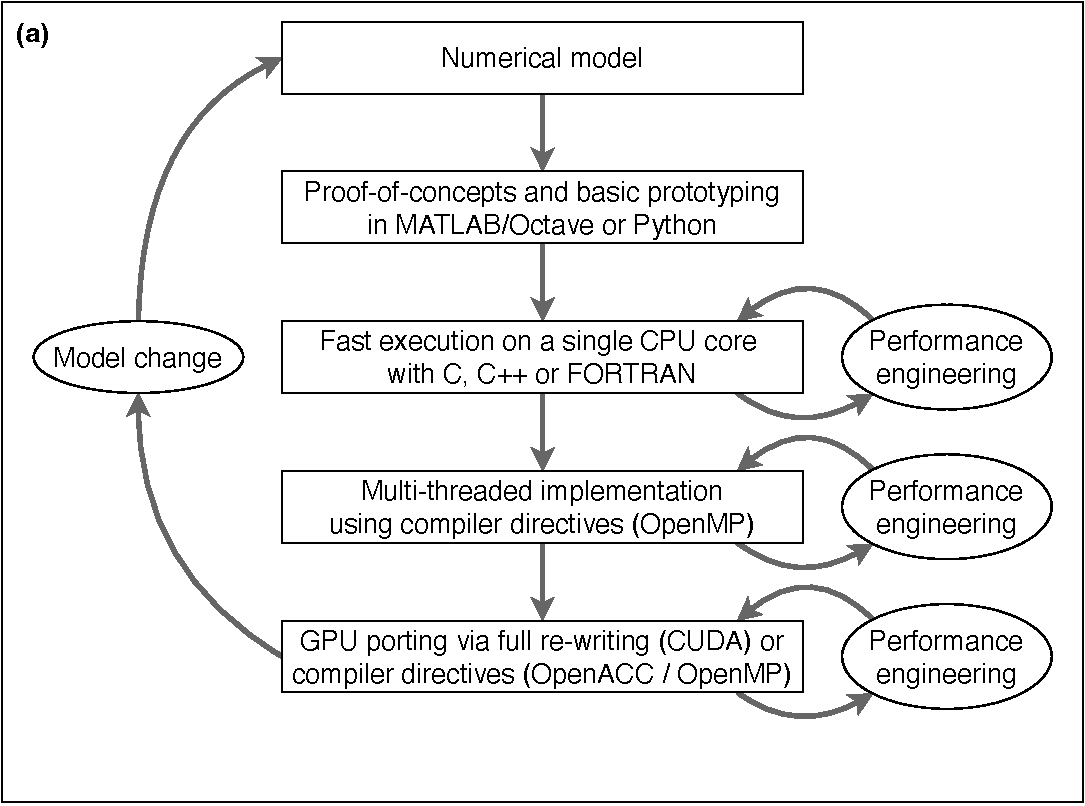
\includegraphics[scale=0.475]{workflow_2.pdf}
		\end{minipage}
		%\hfill
		\begin{minipage}{0.495\textwidth}
			\centering
			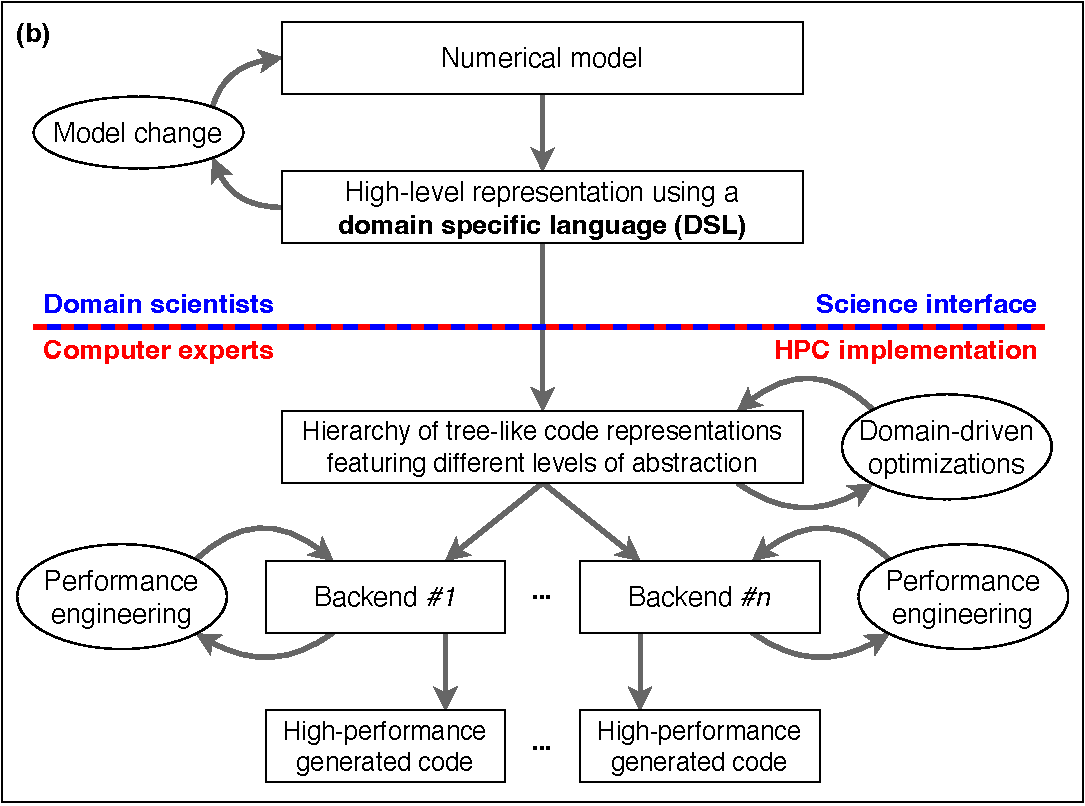
\includegraphics[scale=0.475]{workflow_dsl_2.pdf}
		\end{minipage}

		\caption{Diagrams comparing \textbf{(a)} a well-established workflow in scientific software development, and \textbf{(b)} a DSL-based approach resembling the software engineering strategy advocated in this paper. The red-and-blue dashed line in \textbf{(b)} mark the separation-of-concerns between the domain scientists and the computer experts.}
		\label{fig:dsl}
	\end{figure}

	\subsection{The GT4Py framework}
	\label{section:gt4py}

	GT4Py\footnote{\url{https://github.com/GridTools/gt4py}} is a Python library to generate high-performance implementations of stencil\footnote{A \emph{stencil} is an operator that computes array elements by accessing a fixed pattern of neighbouring items.} kernels as found in weather and climate applications. The library is developed and maintained by the Swiss National Supercomputing Center (CSCS), ETH Zurich, and the Swiss Federal Office of Meteorology and Climatology (MeteoSwiss), and benefits from important contributions by international partners such as the Paul Allen Institute for Artificial Intelligence (AI\textsuperscript{2}). The choice of embedding the GT4Py framework in Python has been mainly dictated by the following factors: (i) Python is taught in many academic courses due its clean, intuitive and expressive syntax, so that a significant fraction of early-career domain scientists \DIFdelbegin \DIFdel{is }\DIFdelend \DIFaddbegin \DIFadd{are }\DIFaddend exposed to the language; (ii) it admits a powerful ecosystem of open source packages for building end-to-end applications; (iii) it is possible to seamlessly interface Python with lower-level languages with minimal overhead and virtually no memory copies; (iv) under the thrust of the Artificial Intelligence and Machine Learning community (AI/ML), the popularity and adoption of Python across the whole scientific community is constantly growing, as opposed to Fortran \citep{shipman23}. The proposed Python implementations of CLOUDSC and CLOUDSC2 are based on the first public release of GT4Py, which only supports Cartesian grids. Latest advancements to support unstructured meshes (contained in the sub-package \pyinline{gt4py.next}) are not discussed in this study.

	\begin{figure}[t!]
		\centering
		\DIFdelbeginFL %DIFDELCMD < 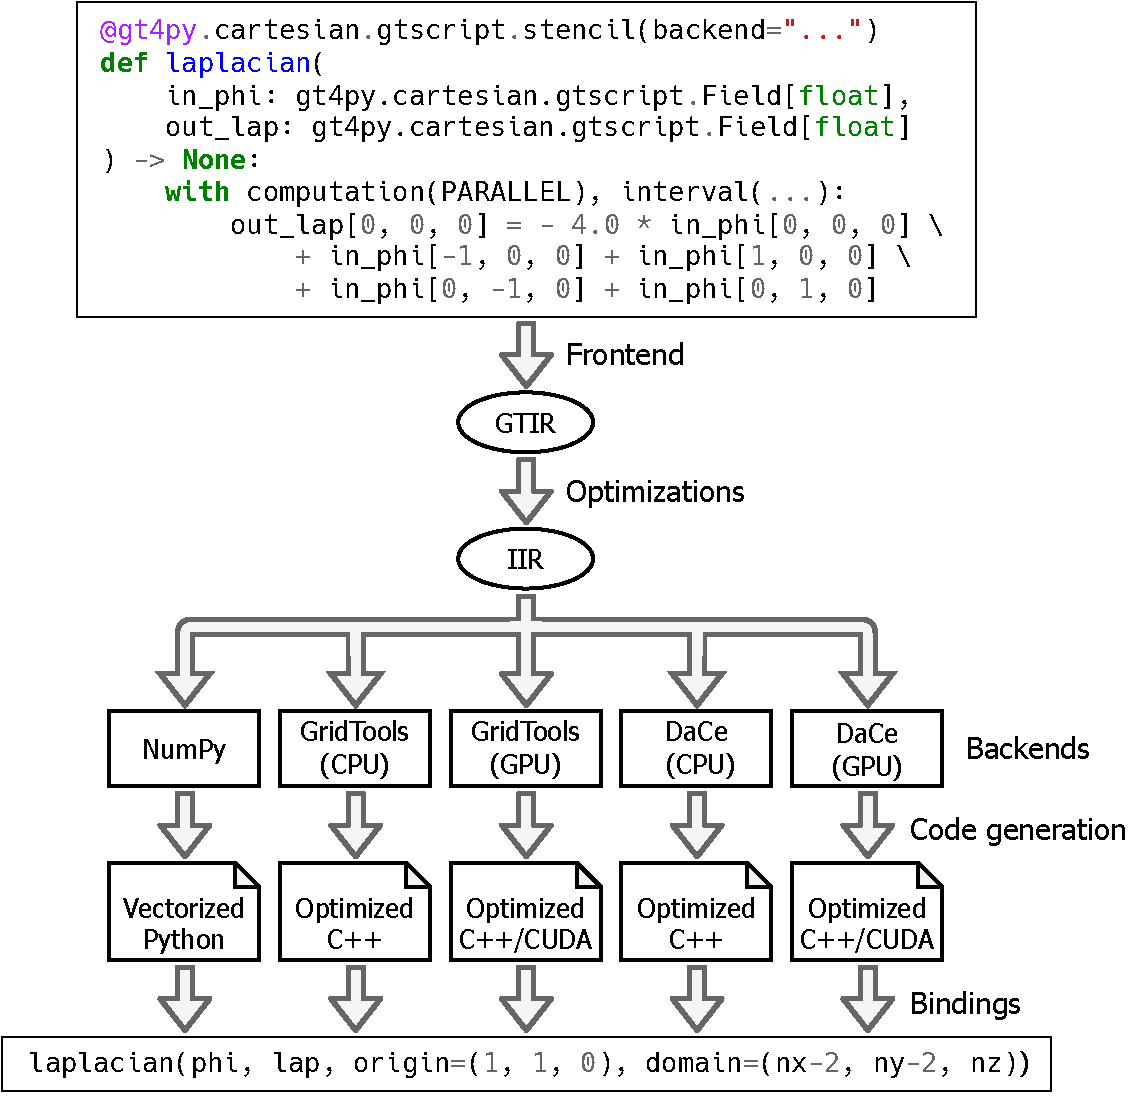
\includegraphics[scale=0.5]{gt4py_2.pdf}
%DIFDELCMD < 		%%%
\DIFdelendFL \DIFaddbeginFL 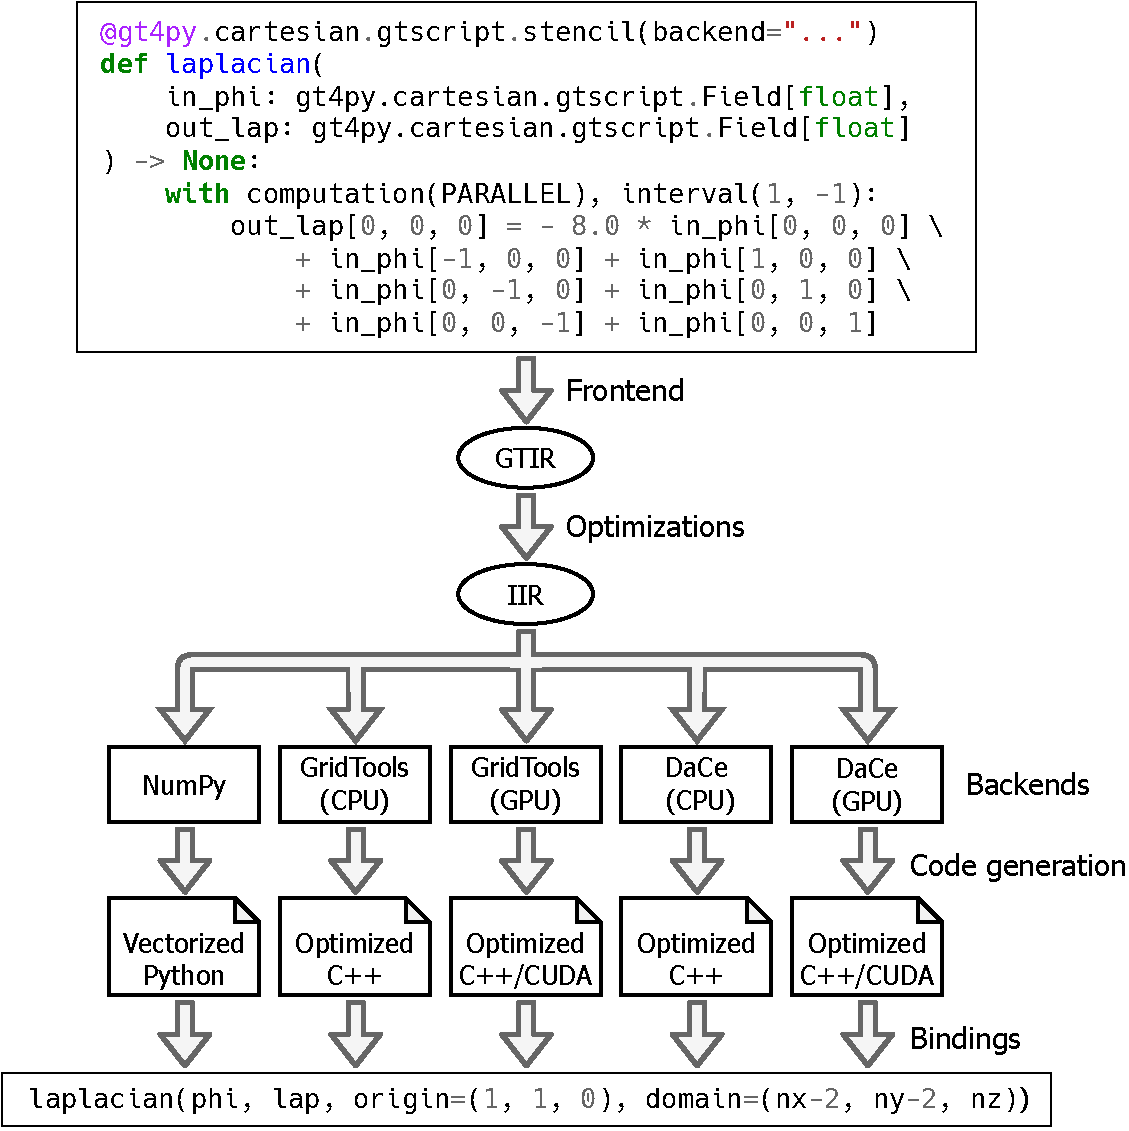
\includegraphics[scale=0.5]{gt4py_3.pdf}
		\DIFaddendFL \caption{Simplified view on the internal stages carried out by the GT4Py toolchain to generate a high-performance CPU or GPU implementation of the \DIFdelbeginFL \DIFdelFL{horizontal }\DIFdelendFL \DIFaddbeginFL \DIFaddFL{three-dimensional }\DIFaddendFL Laplacian stencil starting from its GTScript definition. For the sake of visualization, only two intermediate representations (IRs) are included: the GridTools IR (GTIR) and the Implementation IR (IIR). }
		\label{fig:gt4py}
	\end{figure}

	Figure \ref{fig:gt4py} showcases the main steps undertaken by the GT4Py toolchain to translate the high-level definition of the horizontal Laplacian operator into optimized code, which can be directly called from within Python. The stencil definition is given as a regular Python function using the GTScript DSL. GTScript abstracts \DIFaddbegin \DIFadd{spatial }\DIFaddend for-loops away: computations are described for a single point of a three-dimensional Cartesian grid, and can be \DIFdelbegin \DIFdel{differentiated }\DIFdelend \DIFaddbegin \DIFadd{diversified }\DIFaddend for the vertical boundaries using the \pyinline{interval} context manager. Vertical loops are replaced by \pyinline{computation} contexts, which define the iteration order along the vertical axis: either \pyinline{PARALLEL} (meaning no vertical data dependencies between horizontal planes), \pyinline{FORWARD} or \pyinline{BACKWARD}. Each assignment statement within a computation block can be thought of as a loop over a horizontal plane; no horizontal data dependencies are allowed. Neighbouring points are accessed through relative offsets, with the first two offsets being the horizontal offsets, and the last offset being the vertical offset.

	Any function marked with the \pyinline{gt4py.cartesian.gtscript.stencil} decorator is translated by the GT4Py \emph{frontend} into a hierarchy of tree-like Intermediate Representations (IRs), featuring different levels of abstractions to accommodate diverse optimizations and transformations \citep{gysi21}. The lowest-level IR (denoted as Implementation IR, or IIR) is consumed by the \emph{backends} to generate code that is either optimized for a given architecture or suited to a specific purpose. The following backends are currently available:
	\begin{itemize}
		\item NumPy \citep{harris20} is the \emph{de facto} standard for array computing in Python, and can be used for debugging and fast-prototyping;
		\item GridTools \citep{afanasyev21} is a set of libraries and utilities to write performance-portable applications in the area of weather and climate;
		\item DaCe \citep{ben-nun19} is a parallel programming framework, which internally uses the Stateful DataFlow multiGraph (SDFG) data-centric intermediate representation to decouple domain science and performance engineering.
	\end{itemize}
	The generated code is compiled under the hood, and Python bindings for the resulting executable are automatically produced, so that the stencil can finally be executed by passing the input and output fields and by specifying the origin and size of the computation domain. GT4Py provides convenient utilities to allocate arrays with an optimal memory layout for any given backend, relying on NumPy for CPU storages and CuPy \citep{nishino17} for GPU storages. Concerning GPU computing, we highlight that GT4Py supports both NVIDIA and AMD GPUs.

	A more realistic and pertinent code sample is provided in Listing \ref{lst:saturation-stencil}. It is an abridged GT4Py implementation of the procedure computing the saturation water vapor pressure as a function of air pressure and temperature. The code is extracted from the CLOUDSC2-GT4Py dwarf and highlights two additional features of GTScript: functions and external symbols. Functions can be thought of as macros, and can be used to improve composability, reusability and readability. External symbols are used to encode those scalar parameters (e.g. physical constants) that are kept constant throughout a simulation, and might only change between different model setups. External values must be provided at stencil compilation time. The functionalities provided by the package \pyinline{ifs_physics_common} will be discussed in the following section.

	\begin{listing}[t!]
		\begin{minted}{py}
@gt4py.cartesian.gtscript.function
def \DIFdelbegin \DIFdel{foealfcu}\DIFdelend \DIFaddbegin \DIFadd{foealfa}\DIFaddend (t):
    from __externals__ import \DIFdelbegin \DIFdel{RTICECU}\DIFdelend \DIFaddbegin \DIFadd{RTICE}\DIFaddend , RTWAT, RTWAT_R\DIFdelbegin \DIFdel{TICECU}\DIFdelend \DIFaddbegin \DIFadd{TICE}\DIFaddend _R
    return min(1.0, ((max(\DIFdelbegin \DIFdel{RTICECU}\DIFdelend \DIFaddbegin \DIFadd{RTICE}\DIFaddend , min(RTWAT, t)) - \DIFdelbegin \DIFdel{RTICECU}\DIFdelend \DIFaddbegin \DIFadd{RTICE}\DIFaddend ) * RTWAT_R\DIFdelbegin \DIFdel{TICECU}\DIFdelend \DIFaddbegin \DIFadd{TICE}\DIFaddend _R) ** \DIFdelbegin \DIFdel{2}\DIFdelend \DIFaddbegin \DIFadd{2.0}\DIFaddend )

@gt4py.cartesian.gtscript.function
def foeewmcu(t):
    from __externals__ import R2ES, R3IES, R3LES, R4IES, R4LES, RTT
    return R2ES * (
        foealfcu(t) * exp(R3LES * (t - RTT) / (t - R4LES))
        + (\DIFdelbegin \DIFdel{1 }\DIFdelend \DIFaddbegin \DIFadd{1.0 }\DIFaddend - foealfcu(t)) * (exp(R3IES * (t - RTT) / (t - R4IES)))
    )

@ifs_physics_common.framework.stencil.stencil_collection("saturation")
def saturation(
    in_ap: gtscript.Field[float], in_t: gtscript.Field[float], out_qsat: gtscript.Field[float]
):
    from __externals__ import LPHYLIN, QMAX, R2ES, R3IES, R3LES, R4IES, R4LES, RETV, RTT
    with computation(PARALLEL), interval(...):
        if LPHYLIN:  # linearized physics
            alfa = foealfa(in_t)
            foeewl = R2ES * exp(R3LES * (in_t - RTT) / (in_t - R4LES))
            foeewi = R2ES * exp(R3IES * (in_t - RTT) / (in_t - R4IES))
            foeew = alfa * foeewl + (\DIFdelbegin \DIFdel{1 }\DIFdelend \DIFaddbegin \DIFadd{1.0 }\DIFaddend - alfa) * foeewi
            qs = min(foeew / in_ap, QMAX)
        else:
            ew = foeewmcu(in_t)
            qs = min(ew / in_ap, QMAX)
        out_qsat[0, 0, 0] = qs / (1.0 - RETV * qs)
		\end{minted}

		\caption{GTScript (the Python-embedded DSL exposed by GT4Py) functions and stencil computing the saturation water vapor pressure given the air pressure and temperature. Abridged excerpt from the CLOUDSC2-GT4Py dwarf.}
		\label{lst:saturation-stencil}
	\end{listing}

	% ============================================================
	% section 4
	% ============================================================
	\section{Infrastructure code}
	\label{section:infrastructure-code}

	All stencils of CLOUDSC-GT4Py and CLOUDSC2-GT4Py are defined, compiled and invoked within classes that leverage the functionalities provided by the Sympl package \citep{monteiro18}. Sympl is a toolset of Python utilities to write self-contained and self-documented model components. Because the components share a common Application Public Interface (API), they favor modularity, composability and inter-operability \citep{schaer19}. These aspects are of utter importance, for instance, when it comes to assessing the impact of process coupling on weather forecasts and climate projections \citep{ubbiali21}.

	\begin{listing}[t!]
		\begin{minted}{py}
import cupy as cp
from functools import cached_property
import numpy as np
from typing import Optional, Union
from ifs_physics_common.framework.components import DiagnosticComponent
from ifs_physics_common.framework.config import GT4PyConfig
from ifs_physics_common.framework.grid import ComputationalGrid, I, J, K

# type alias originally defined in ifs_physics_common.utils.typingx
StorageDict = dict[str, Union[cp.ndarray. np.ndarray]]

class Saturation(DiagnosticComponent):
    def __init__(
        self,
        computational_grid: ComputationalGrid,
        lphylin: bool,
        yoethf_parameters: Optional[dict[str, float]] = None,
        yomcst_parameters: Optional[dict[str, float]] = None,
        gt4py_config: GT4PyConfig,
    ) -> None:
        super().__init__(computational_grid, gt4py_config)
        externals = {"LPHYLIN": lphylin, "QMAX": 0.5}
        externals.update(yoethf_parameters or {})
        externals.update(yomcst_parameters or {})
        self.saturation = self.compile_stencil("saturation", externals)

    @cached_property
    def _input_properties(self):
        return {"ap": {"grid": (I, J, K), "units": "Pa"}, "t": {"grid": (I, J, K), "units": "K"}}

    @cached_property
    def _diagnostic_properties(self):
        return {"qsat": {"grid": (I, J, K), "units": "g g^-1"}}

    def array_call(self, state: StorageDict, out: StorageDict) -> None:
        self.saturation(
            in_ap=state["ap"],
            in_t=state["t"],
            out_qsat=out["qsat"],
            origin=(0, 0, 0),
            domain=self.computational_grid.grids[I, J, K].shape,
        )
		\end{minted}

		\caption{A Python class to compute the saturation water vapor pressure given the air pressure and temperature. Abridged excerpt from the CLOUDSC2-GT4Py dwarf.}
		\label{lst:saturation-infrastructure}
	\end{listing}

	Sympl components interact through dictionaries whose keys are the names of the model variables (fields), and whose values are xarray's \pyinline{DataArray}s \citep{hoyer17} collecting the grid point values, the labelled dimensions, the axis coordinates, and the units for those variables. The most relevant component exposed by Sympl is \pyinline{TendencyComponent}, producing tendencies for prognostic variables and retrieving diagnostics. The class defines a minimal interface to declare the list of input and output fields, and initialize and run an instance of the class. This imposes minor constraints on model developers when writing a new physics package.

	The bespoke infrastructure code for CLOUDSC-GT4Py and CLOUDSC2-GT4Py is bundled as an installable Python package called \pyinline{ifs_physics_common}. Not only \DIFdelbegin \DIFdel{it builds }\DIFdelend \DIFaddbegin \DIFadd{does it build }\DIFaddend upon Sympl, but \DIFdelbegin \DIFdel{is }\DIFdelend also extends it with grid-aware and stencil-oriented functionalities. Both the CLOUDSC cloud microphysics and the non-linear, tangent-linear and adjoint formulations of CLOUDSC2 are encoded as stand-alone \pyinline{TendencyComponent} classes settled over a \pyinline{ComputationalGrid}. The latter is a collection of index spaces for different grid locations. For instance, \pyinline{(I, J, K)} corresponds to cell centers, while \pyinline{(I, J, K-1/2)} denotes vertically-staggered grid points. For any input and output field, its name, units and grid location are specified as class properties. When running the component via the \emph{dunder} method \pyinline{__call__}, Sympl transparently extracts the raw data from the input \pyinline{DataArray}s according to the information provided in the class definition. This step may involve units conversion and axis transposition. The resulting storages are forwarded to the method \pyinline{array_call}, which carries out the actual computations, possibly by executing GT4Py stencil kernels.

	Listing \ref{lst:saturation-infrastructure} brings a concrete example from CLOUDSC2-GT4Py: a model component leveraging the stencil defined in Listing \ref{lst:saturation-stencil} to compute the saturation water vapor pressure. The class inherits \pyinline{DiagnosticComponent}, a stripped-down version of \pyinline{TendencyComponent}, which only retrieves diagnostic quantities. Within the instance initializer \pyinline{__init__}, the stencil from Listing \ref{lst:saturation-stencil}, registered using the decorator \pyinline{ifs_physics_common.framework.stencil.stencil_collection}, is compiled using the utility method \pyinline{compile_stencil}. The options configuring the stencil compilation (e.g.\,the GT4Py backend) are fetched from the dataclass \pyinline{GT4PyConfig}.

	% ============================================================
	% section 5
	% ============================================================
	\section{Performance analysis}
	\label{section:performance-analysis}

	In this section, we highlight the results from a comprehensive performance testing. We compare the developed CLOUDSC-GT4Py and CLOUDSC2-GT4Py codes against reference Fortran versions and various other programming prototypes. The simulations were performed on three different supercomputers:
	\begin{itemize}
		\item[(i)] Piz Daint\footnote{\url{https://www.cscs.ch/computers/piz-daint}}, an HPE Cray XC40/XC50 system installed at CSCS in Lugano, Switzerland;
		\item[(ii)] MeluXina\footnote{\url{https://docs.lxp.lu/}}, an ATOS BullSequana XH2000 machine hosted by LuxConnect in Bissen, Luxembourg, and procured by the EuroHPC Joint Undertaking (JU) initiative;
		\item[(iii)] the Cray HPE EX235a supercomputer LUMI\footnote{\url{https://docs.lumi-supercomputer.eu/}}, an EuroHPC pre-exascale machine at the Science Information Technology Center (CSC) in Kajaani, Finland.
	\end{itemize}
	On each machine, the CLOUDSC and CLOUDSC2 applications are executed on a single hybrid node, that sports one or multiple GPU accelerators alongside the host CPU. An overview of the node architectures for the three considered supercomputers can be found in Table \ref{tab:architecture}.

	\begin{table}[t!]
		\setlength\extrarowheight{2pt}
		\centering
		\begin{tabular}{|c|c|c|c|c|}
			\hline
			\textbf{System} & \textbf{CPU} & \textbf{GPU} & \textbf{RAM} & \textbf{NUMA domains} \\
			\hline
			Piz Daint & 1x Intel Xeon E5-2690v3 12c & 1x NVIDIA Tesla P100 16GB & 64 GB & 1 \\
			MeluXina & 2x AMD EPYC Rome 7452 32c & 4x NVIDIA Tesla A100 40GB & 512 GB & 4 \\
			LUMI & 1x AMD EPYC Trento 7A53 64c & 4x AMD Instinct MI250X & 512 GB & 8 \\
			\hline
		\end{tabular}
		\vspace*{0.2cm}
		\caption{Overview of the node architecture for the hybrid partition of Piz Daint, MeluXina and LUMI. Only the technical specifications which are most relevant for the purposes of this paper are reported.}
		\label{tab:architecture}
	\end{table}

	Besides the GT4Py codes, we involve up to four alternative lower-level programming implementations, which will be documented in an upcoming publication.
	\begin{itemize}
		\item[(a)] The baseline Fortran version, enriched with OpenMP directives for multi-threading execution on CPU.
		\item[(b)] An optimized GPU-enabled version based on OpenACC using the single-column coalesced (SCC) loop layout in combination with loop fusion and temporary local array demotion (so-called ``k-caching''). While the SCC loop layout yields more efficient access to device memory and increased parallelism, the k-caching technique significantly reduces register pressure and memory traffic. This is achieved via loop fusion to eliminate most loop-carried dependencies and consequently allows to demote temporaries to scalars.
		\item[(c)] The currently best-performing Loki generated and GPU-enabled variant.
		\item[(d)] An optimized GPU-enabled version of CLOUDSC including k-caching. The code is written either in CUDA or HIP, to target both NVIDIA GPUs (shipped with Piz Daint and MeluXina) and AMD GPUs (available on LUMI).
	\end{itemize}

	\begin{table}[t!]
		\renewcommand{\arraystretch}{1.4}
		\centering
		\begin{footnotesize}
			\begin{tabular}{|c|c|c|c|c|}
				\hline
				& \textbf{Implementation} & \textbf{CLOUDSC} & \textbf{CLOUDSC2: Non-linear} & \textbf{CLOUDSC2: Symmetry test} \\
				\hline
				\multirow{6}{*}{\rotatebox[origin=c]{90}{\textbf{Piz Daint}}} & Fortran: OpenMP (CPU) & Intel Fortran 2021.3.0 & Intel Fortran 2021.3.0 & Intel Fortran 2021.3.0 \\
				& Fortran: OpenACC (GPU) & NVIDIA Fortran 21.3-0 & - & - \\
				& Fortran: Loki (GPU) & NVIDIA Fortran 21.3-0 & NVIDIA Fortran 21.3-0 & - \\
				& C: CUDA (GPU) & NVIDIA CUDA 11.2.67 & - & - \\
				& GT4Py: CPU k-first & g++ (GCC) 10.3.0 & g++ (GCC) 10.3.0 & g++ (GCC) 10.3.0 \\
				& GT4Py: DaCe (GPU) & NVIDIA CUDA 11.2.67 & NVIDIA CUDA 11.2.67 & NVIDIA CUDA 11.2.67 \\
				\hline
				\multirow{6}{*}{\rotatebox[origin=c]{90}{\textbf{MeluXina}}} & Fortran: OpenMP (CPU) & NVIDIA Fortran 22.7-0 & NVIDIA Fortran 22.7-0 & - \\
				& Fortran: OpenACC (GPU) & NVIDIA Fortran 22.7-0 & - & - \\
				& Fortran: Loki (GPU) & NVIDIA Fortran 22.7-0 & NVIDIA Fortran 22.7-0 & - \\
				& C: CUDA (GPU) & NVIDIA CUDA 11.7.64 & - & - \\
				& GT4Py: CPU k-first & g++ (GCC) 11.3.0 & g++ (GCC) 11.3.0 & g++ (GCC) 11.3.0 \\
				& GT4Py: DaCe (GPU) & NVIDIA CUDA 11.7.64 & NVIDIA CUDA 11.7.64 & NVIDIA CUDA 11.7.64 \\
				\hline
				\multirow{6}{*}{\rotatebox[origin=c]{90}{\textbf{LUMI}}} & Fortran: OpenMP (CPU) & ~~ Cray Fortran 14.0.2 ~~ & Cray Fortran 14.0.2 & Cray Fortran 14.0.2 \\
				& Fortran: OpenACC (GPU) & Cray Fortran 14.0.2 & - & - \\
				& Fortran: Loki (GPU) & Cray Fortran 14.0.2 & Cray Fortran 14.0.2 & - \\
				& C: HIP (GPU) & Cray C/C++ 15.0.1 & - & - \\
				& GT4Py: CPU k-first & Cray C/C++ 15.0.1 & Cray C/C++ 15.0.1 & Cray C/C++ 15.0.1 \\
				& GT4Py: DaCe (GPU) & Cray C/C++ 15.0.1 & Cray C/C++ 15.0.1 & Cray C/C++ 15.0.1 \\
				\hline
			\end{tabular}
		\end{footnotesize}
		\vspace*{0.2cm}
		\caption{For each coding version of the CLOUDSC and CLOUDSC2 dwarfs considered in the performance analysis, the table reports the compiler suite used to compile the codes on Piz Daint, MeluXina and LUMI. The codes are compiled with all major optimization options enabled. Those implementations which are either not available or not working are marked with a dash; more details, as well as a high-level description of each coding implementation, are provided in the text.}
		\label{tab:compiler}
	\end{table}

	\noindent Table \ref{tab:compiler} documents the compiler specifications employed for each of the programming implementations, on Piz Daint, MeluXina and LUMI. We consistently apply the most aggressive optimization, ensuring that the underlying code manipulations do not harm validation. For the different algorithms at consideration, validation is carried out as follows.
	\begin{itemize}
		\item For CLOUDSC and CLOUDSC2NL, the results from each coding version are directly compared with serialized reference data produced on the CPU. For each output field, we perform an element-wise comparison using the NumPy function \pyinline{allclose}\footnote{\url{https://numpy.org/devdocs/reference/generated/numpy.allclose.html}}. Specifically, the GT4Py rewrites validate on both CPU and GPU with an absolute and relative tolerance of $10^{-12}$ and $10^{-18}$ when employing double precision. When reducing the precision to 32-bits, the absolute and relative tolerance levels need to be increased to $10^{-4}$ and $10^{-7}$ on CPU, and $10^{-2}$ and $10^{-7}$ on GPU. In the latter case, we observe that the field representing the enthalpy flux of ice still does not pass validation. We attribute the larger deviation from the baseline data on the device to the different instruction sets underneath CPUs and GPUs.
		\item All implementations of CLOUDSC2TL and CLOUDSC2AD are validated using the Taylor test (cf.\,Algorithm \ref{alg:taylor-test}) and the symmetry test (cf.\,Algorithm \ref{alg:symmetry-test}), respectively. \DIFdelbegin \DIFdel{However, the }\DIFdelend \DIFaddbegin \DIFadd{In this respect, we emphasize that the GT4Py implementations satisfy the }\DIFaddend conditions of both tests \DIFdelbegin \DIFdel{are not satisfied when using single precision . This is not surprising, since both tests are highly sensitive to round-off errors.
	Nevertheless, performance numbers for the execution of the algorithms were taken.
	}\DIFdelend \DIFaddbegin \DIFadd{on all considered computing architectures, regardless of whether double or single precision is employed.
	}\DIFaddend \end{itemize}
	\noindent The source repositories for CLOUDSC and CLOUDSC2 dwarfs may include multiple variants of each reference implementation, varying for the optimization strategies. In our analysis, we always take into account the fastest variant of each alternative implementation; for the sake of reproducibility, Table \ref{tab:versions} contains the strings identifying the coding versions at consideration and the corresponding NPROMA\DIFaddbegin \footnote{\DIFadd{NPROMA slicing is a cache blocking technique adopted in all Fortran codes considered in this paper. Given a two-dimensional array shaped $(K * M, \, N)$, this is re-arranged as a three-dimensional array shaped $(K, \, M, \, N)$. The leading dimension of the three-dimensional array is commonly called ``NPROMA'', with $K$ being the ``NPROMA blocking factor''. For the sake of brevity, in the text we indicate $K$ simply as ``NPROMA''. For an insightful discussion on the NPROMA slicing technique, we refer the readers to, e.g., \mbox{%DIFAUXCMD
\citet{muller19} }\hskip0pt%DIFAUXCMD
and \mbox{%DIFAUXCMD
\citet{bauer20}}\hskip0pt%DIFAUXCMD
.}} \DIFaddend employed in the runs. \DIFaddbegin \DIFadd{Similarly, for all Python implementations we consider only the most performant backends of GT4Py: the GridTools C++ CPU backend with k-first memory layout, and the DaCe GPU backend.
}\DIFaddend 

	\begin{table}[t!]
		\renewcommand{\arraystretch}{1.4}
		\centering
		\begin{footnotesize}
			\begin{tabular}{|c|c|c|c|c|}
				\hline
				& \textbf{Implementation} & \textbf{CLOUDSC} & \textbf{CLOUDSC2: Non-linear} & \textbf{CLOUDSC2: Symmetry test} \\
				\hline
				\multirow{4}{*}{\rotatebox[origin=c]{90}{\textbf{Piz Daint}}} & Fortran: OpenMP (CPU) & \texttt{fortran} (32) & \texttt{nl} (32) & \texttt{ad} (32) \\
				& Fortran: OpenACC (GPU) & \texttt{gpu-scc-k-caching} (128) & - & - \\
				& Fortran: Loki (GPU) & \texttt{loki-scc-cuf-hoist} (128) & \texttt{nl-loki-scc-hoist} (64) & - \\
				& C: CUDA (GPU) & \texttt{cuda-k-caching} (128) & - & - \\
				\hline
				\multirow{4}{*}{\rotatebox[origin=c]{90}{\textbf{MeluXina}}} & Fortran: OpenMP (CPU) & \texttt{fortran} (32) & \texttt{nl} (32) & - \\
				& Fortran: OpenACC (GPU) & \texttt{gpu-scc-k-caching} (128) & - & - \\
				& Fortran: Loki (GPU) & \texttt{loki-scc-cuf-hoist} (128) & \texttt{nl-loki-scc-hoist} (128) & - \\
				& C: CUDA (GPU) & \texttt{cuda-k-caching} (128) & - & - \\
				\hline
				\multirow{4}{*}{\rotatebox[origin=c]{90}{\textbf{LUMI}}} & Fortran: OpenMP (CPU) & ~~ \texttt{fortran} (32) ~~ & \texttt{nl} (32) & \texttt{ad} (32) \\
				& Fortran: OpenACC (GPU) & \texttt{gpu-scc-k-caching} (256) & - & - \\
				& Fortran: Loki (GPU) & \texttt{loki-scc-hoist} (256) & \texttt{nl-loki-scc-hoist} (256) & - \\
				& C: HIP (GPU) & \texttt{hip-k-caching} (64) & - & - \\
				\hline
			\end{tabular}
		\end{footnotesize}
		\vspace*{0.2cm}
		\caption{For each reference implementation of the CLOUDSC and CLOUDSC2 dwarfs, the table reports the string identifying the specific variant considered in the performance analysis on Piz Daint, MeluXina and LUMI. The corresponding NPROMA is provided within parentheses. Those implementations which are either not available or not working are marked with a dash.}
		\label{tab:versions}
	\end{table}

	\begin{figure}[t!]
		\centering
		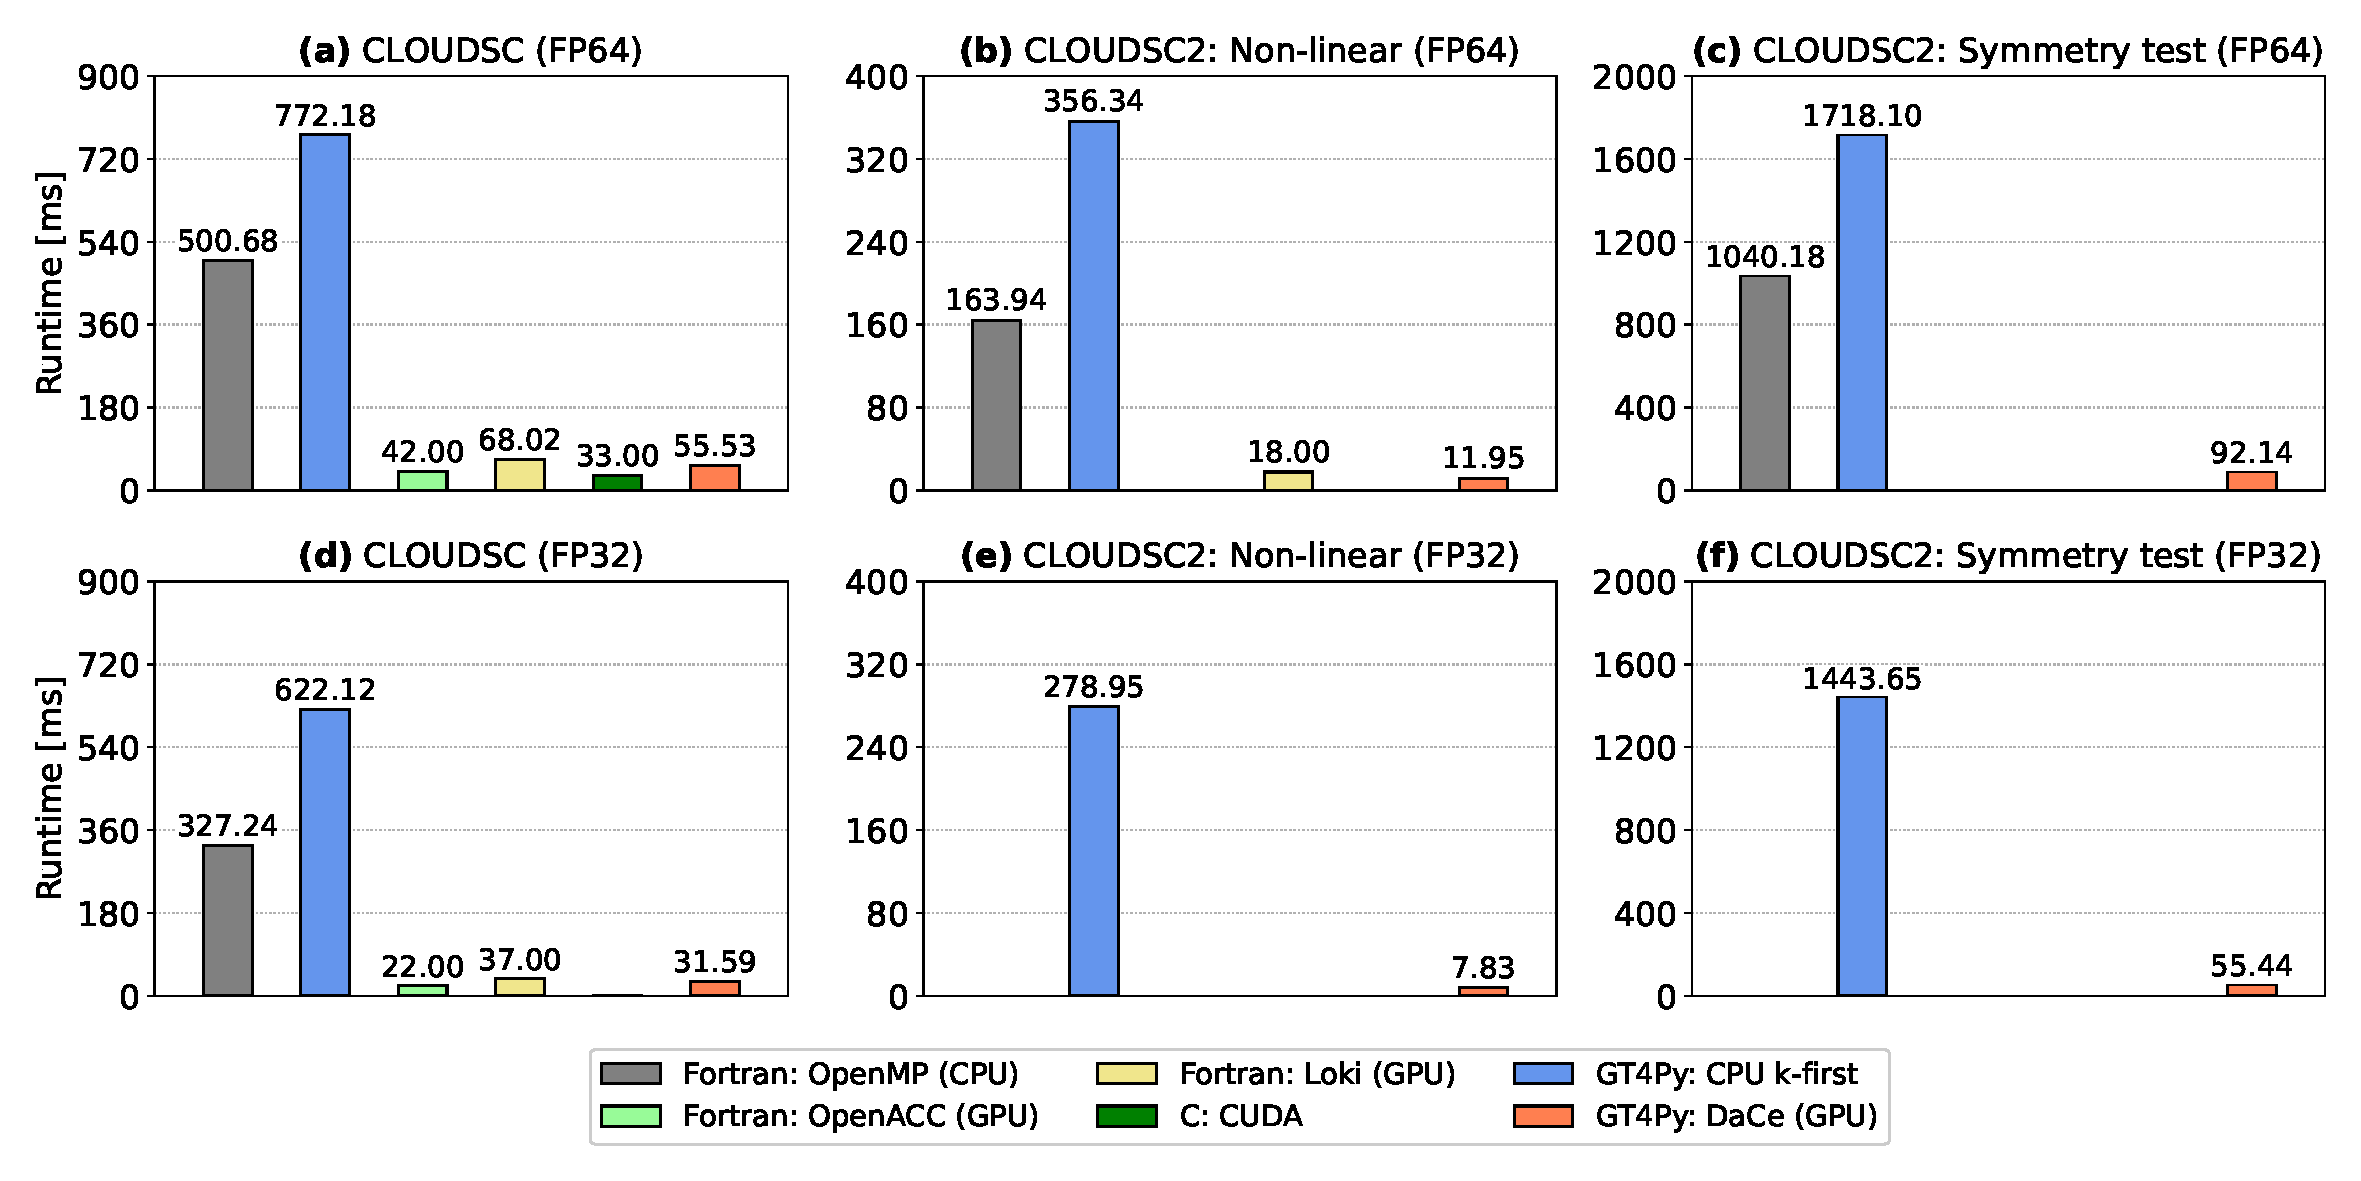
\includegraphics[scale=0.44]{performance_daint_2.pdf}
		\caption{Execution time on a single NUMA domain of a hybrid node of the Piz Daint supercomputer for CLOUDSC (left column), CLOUDSC2NL (center column) and the symmetry test for CLOUDSC2TL and CLOUDSC2AD (right column) using either double precision (top row) or single precision (bottom row) floating point arithmetic. The computational domain consists of 65536 columns and 137 vertical levels. Displayed are the multi-threaded Fortran baseline using OpenMP (grey); two GPU-accelerated Fortran implementations, either using OpenACC directives (lime) or the source-to-source translation tool Loki (yellow); an optimized CUDA C version (green); and the GT4Py rewrite, either using the GridTools C++ CPU backend with k-first data ordering (blue) or the DaCe GPU backend (orange). All numbers should be interpreted as an average over $50$ realizations. The panels only show the code versions available and validating at the time of writing.}
		\label{fig:performance-daint}
	\end{figure}

	\noindent For the interpretation of the CPU versus GPU performance numbers, we note that host codes are executed on all the cores available on a single Non-Uniform Memory Access (NUMA) domain of a compute node, while device codes are launched on the GPU attached to that NUMA domain. In a distributed-memory context, this choice allows to fit the same number of MPI ranks per node, either on CPU or GPU. Table \ref{tab:architecture} reports the number of NUMA partitions per node for Piz Daint, MeluXina and LUMI, with the compute and memory resources being evenly distributed across the NUMA domains. Note that the compute nodes of the GPU partition of LUMI have the low-noise mode activated, which reserves one core per NUMA domain to the operating system, so that only 7 out of 8 cores are available to the jobs. Moreover, \DIFaddbegin \DIFadd{we highlight that }\DIFaddend each MI250X GPU \DIFdelbegin \DIFdel{is split into two }\DIFdelend \DIFaddbegin \DIFadd{consists of two Graphics Compute Dies (GCDs) connected via four AMD Infinity Fabric links but not sharing physical memory. From a software perspective, each compute node of LUMI is equipped with 8 }\DIFaddend virtual GPUs (vGPUs), with each vGPU \DIFaddbegin \DIFadd{corresponding to a single GCD and }\DIFaddend assigned to a different NUMA domain.

	\begin{figure}[t!]
		\centering
		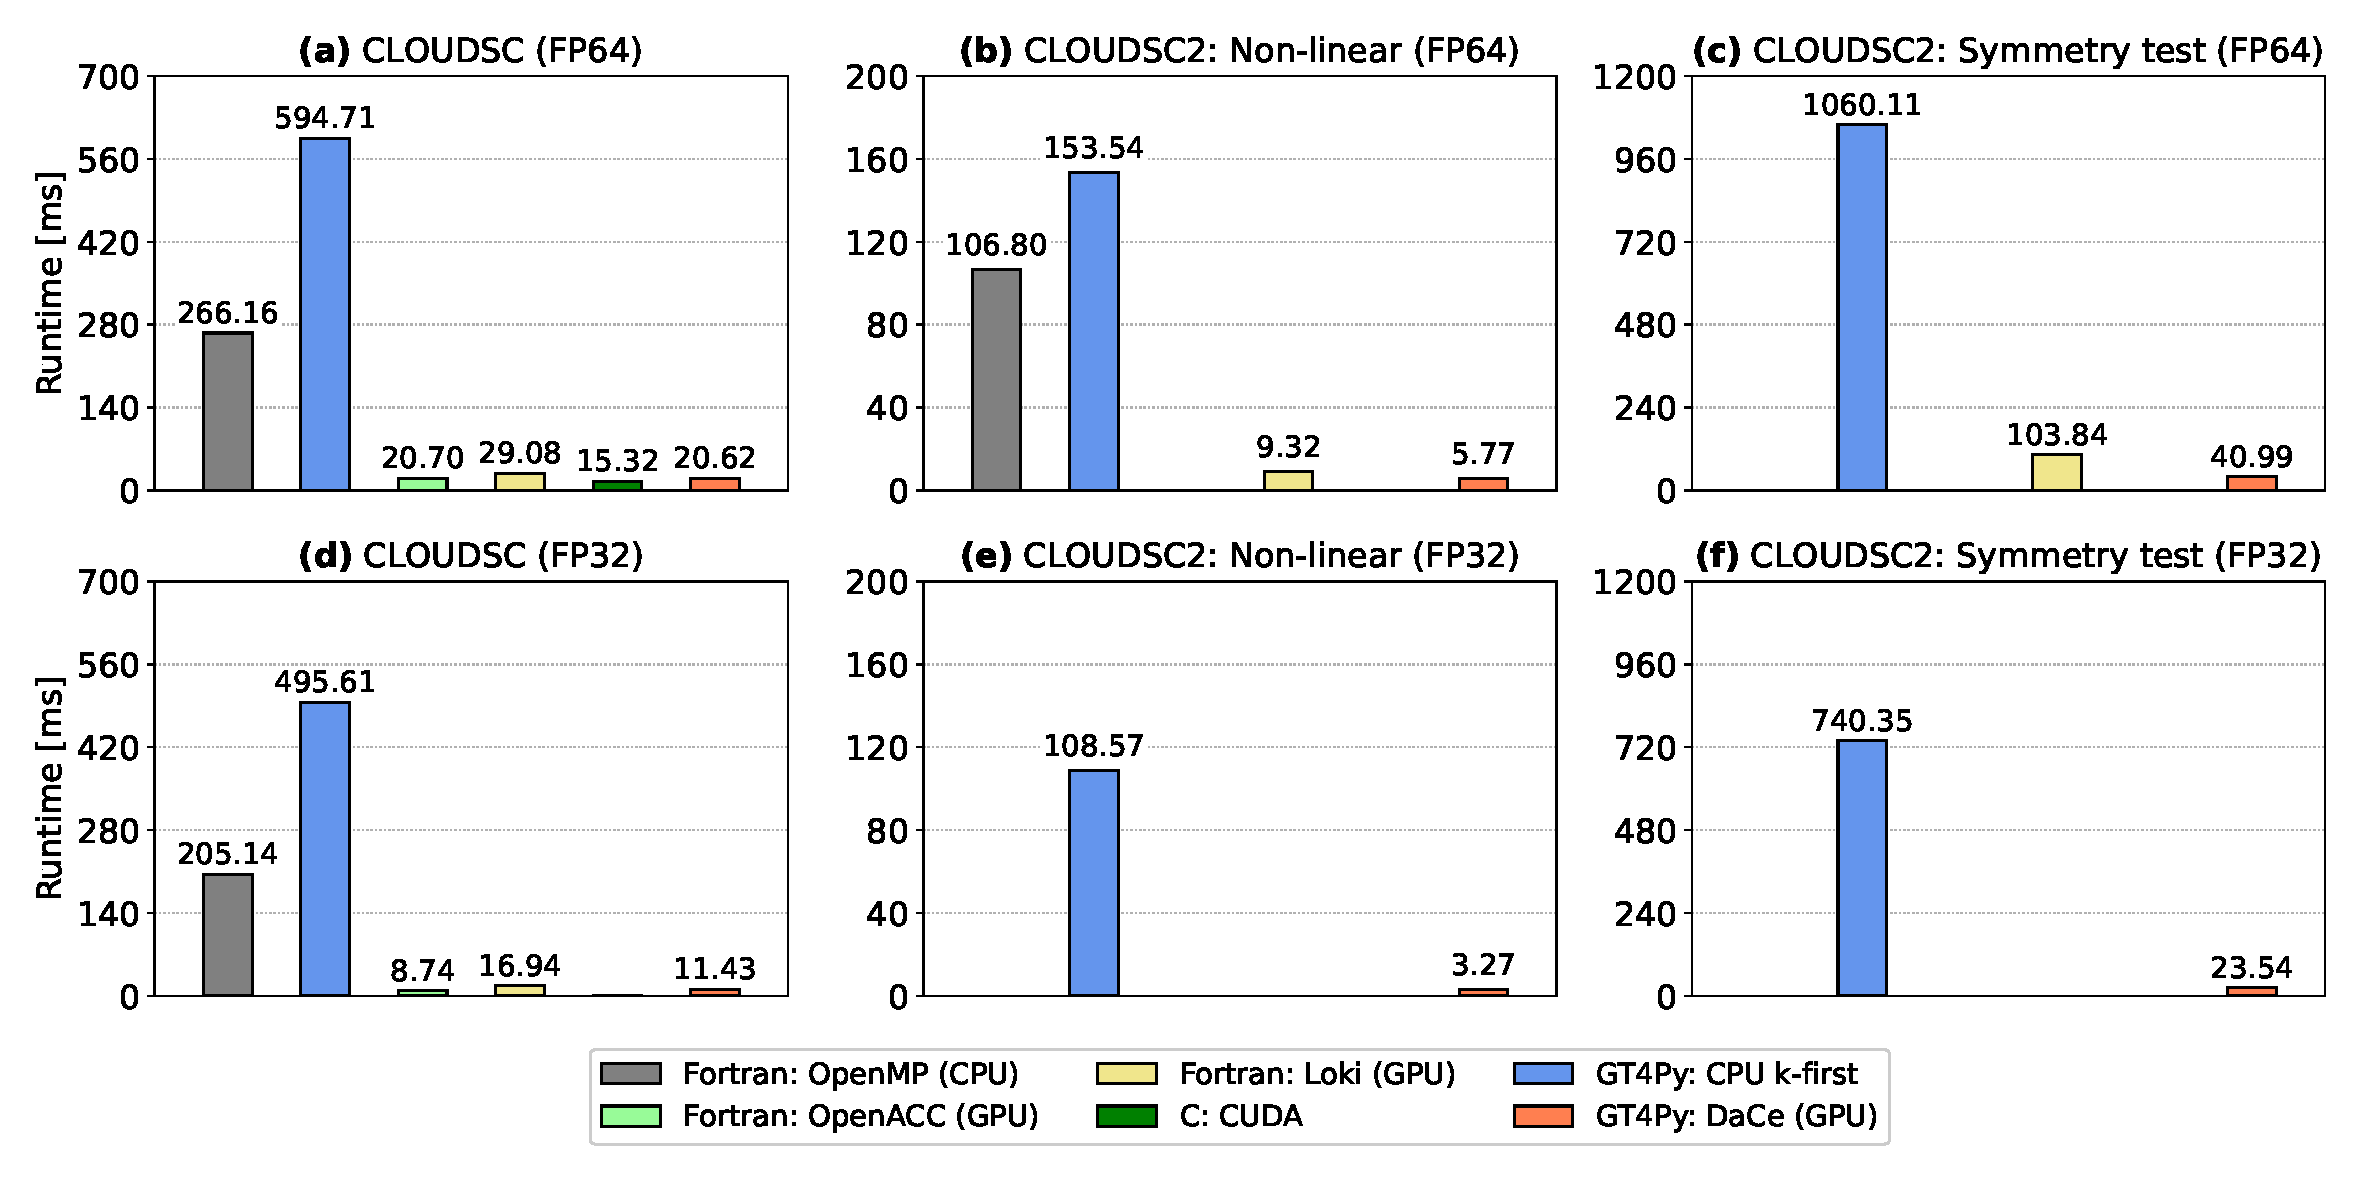
\includegraphics[scale=0.44]{performance_mlux_2.pdf}
		\caption{As Fig.\,\ref{fig:performance-daint} but for the MeluXina supercomputer.}
		\label{fig:performance-mlux}
	\end{figure}

	Figures \ref{fig:performance-daint}-\ref{fig:performance-lumi} visualize the execution times for CLOUDSC (left column), CLOUDSC2NL  (center column) and the symmetry test for CLOUDSC2TL and CLOUDSCAD (right column) for Piz Daint, MeluXina and LUMI, respectively\DIFaddbegin \footnote{\DIFadd{When measuring the performance of the symmetry test, the validation procedure -- corresponding to lines 11-23 of Algorithm \ref{alg:symmetry-test} -- is switched off.}}\DIFaddend . All performance numbers refer to a grid size of 65536 columns, with each column featuring 137 vertical levels. In each figure, execution times are provided for simulations running either entirely in double precision (\DIFaddbegin \DIFadd{corresponding to the 64-bit IEEE format and denoted as }\DIFaddend FP64; top row) or in single precision (\DIFaddbegin \DIFadd{corresponding to the 32-bit IEEE format and denoted as }\DIFaddend FP32; bottom row). Within each panel, the plotted bars reflect the execution time of the various codes, with a missing bar indicating the corresponding code (non-GT4Py) is either not available or not working properly. Specifically,
	\begin{itemize}
		\item the Fortran version of CLOUDSC2AD can only run on a single OpenMP thread on MeluXina (the issue is still under investigation);
		\item a native GPU-enabled version of CLOUDSC using 32-bit floating point arithmetic does not exist at the time of writing, and no CUDA/HIP implementations are available for CLOUDSC2;
		\item all Fortran-based implementations of the three formulations of CLOUDSC2 can only use double precision computations;
		\item a Loki version of CLOUDSC2TL and CLOUDSC2AD is not available at the time of writing.
	\end{itemize}

	\noindent Notably, we find the GT4Py rewrite of both CLOUDSC and CLOUDSC2 to be very robust, as the codes execute on every CPU and GPU architecture included in the study, and can always employ either double or single precision floating point arithmetic. With GT4Py, changing the backend with the respective target architecture, or changing the precision of computations, is as easy as setting a namelist parameter. Moreover, at the time of writing the GT4Py implementations of the more complex tangent-linear and adjoint formulations of CLOUDSC2 were the first codes enabling GPU execution, again both in double or single precision.

	\begin{figure}[t!]
		\centering
		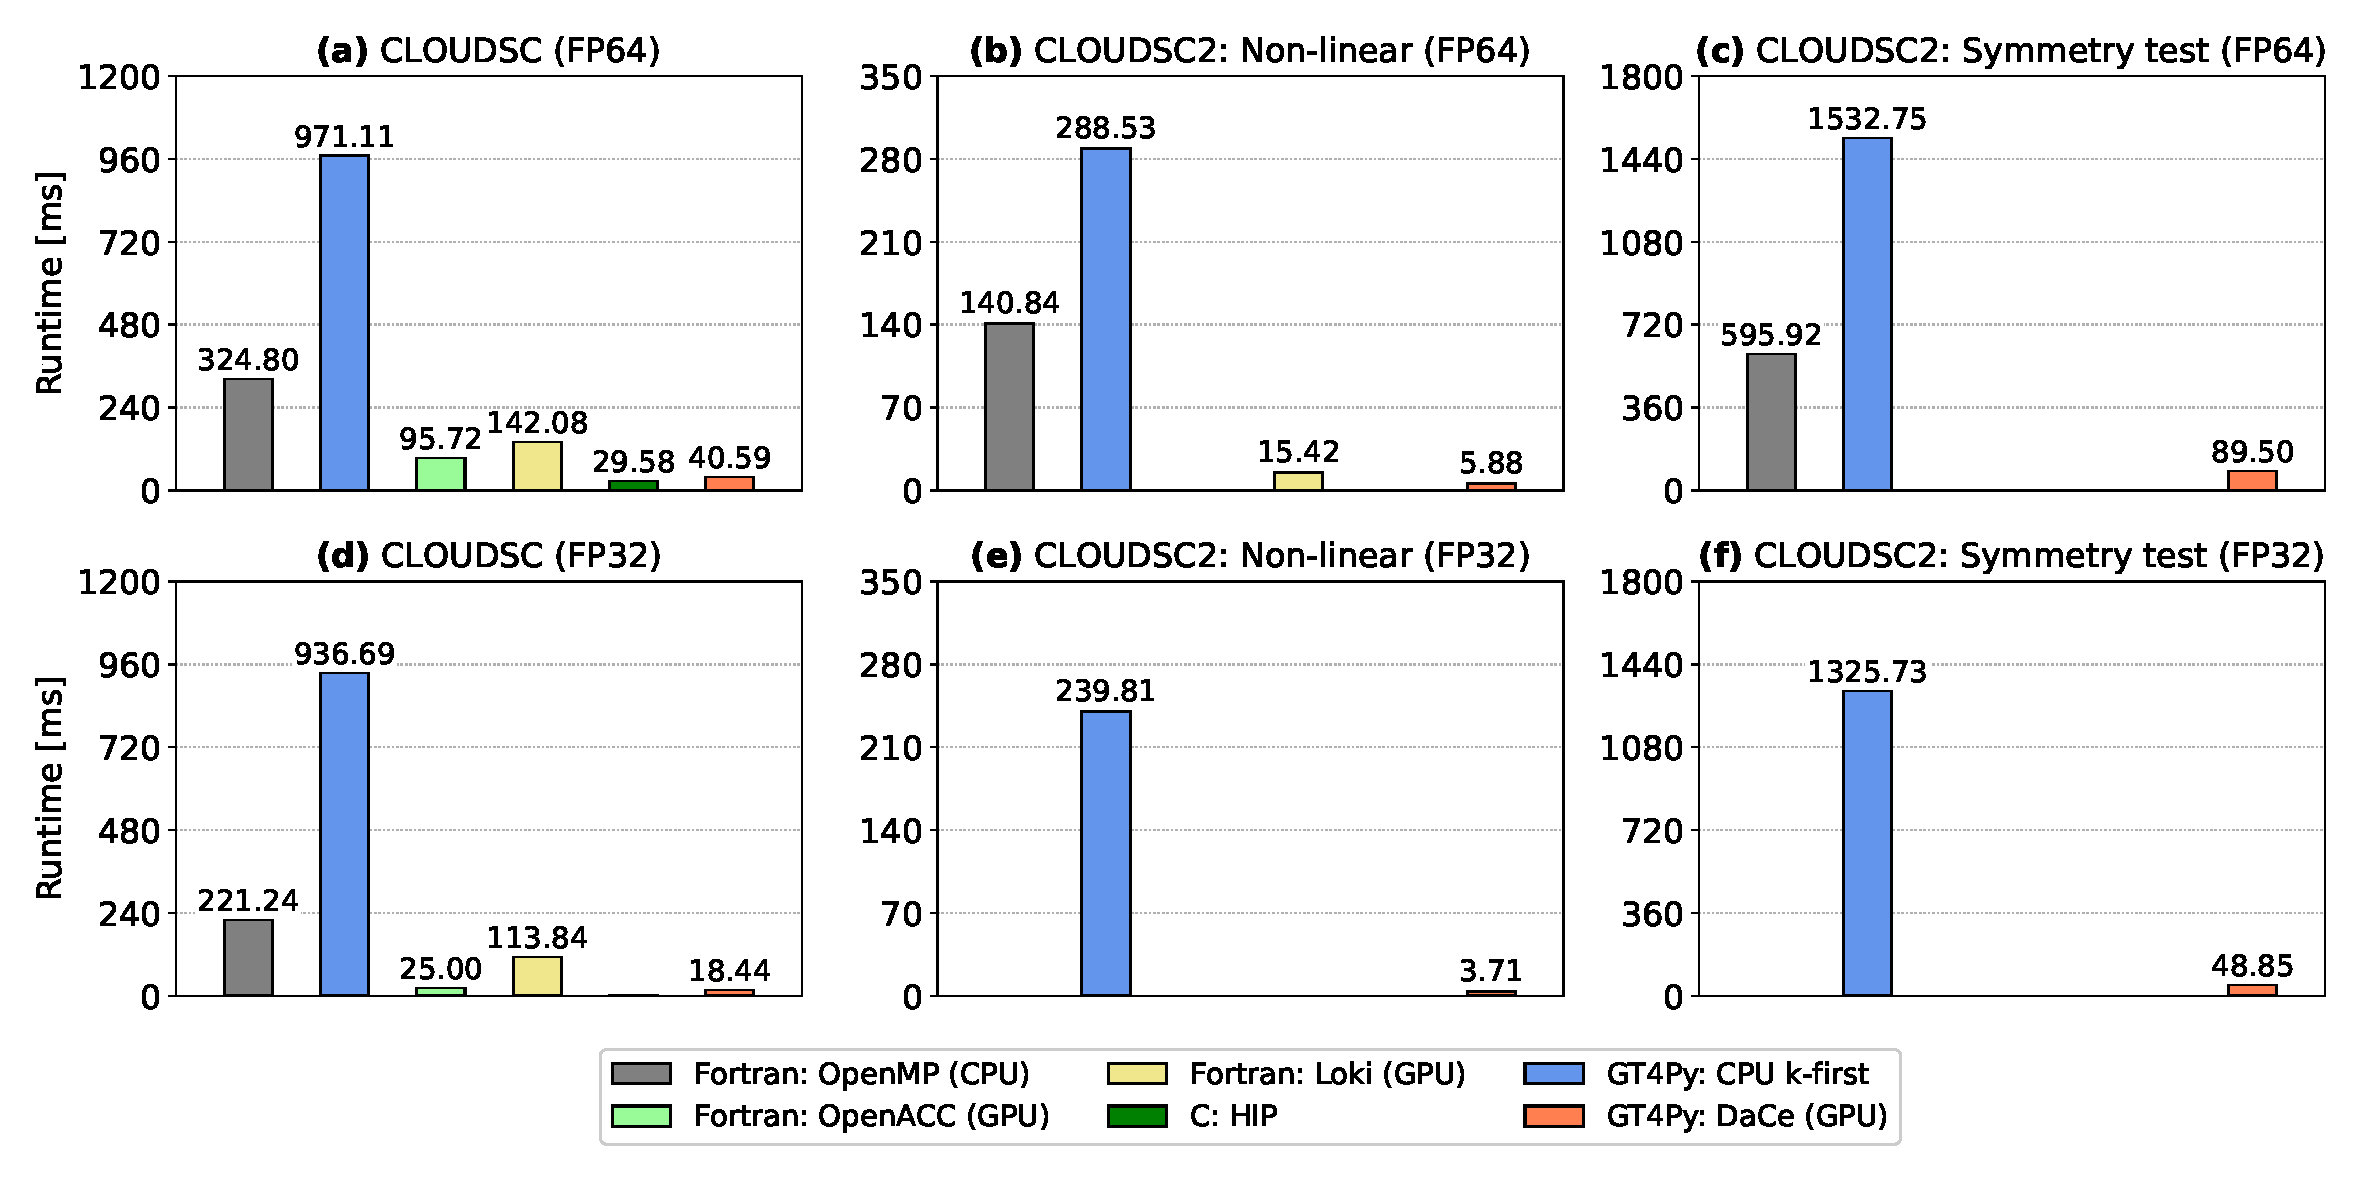
\includegraphics[scale=0.44]{performance_lumi_2.pdf}
		\caption{As Fig.\,\ref{fig:performance-daint} but for the LUMI supercomputer.}
		\label{fig:performance-lumi}
	\end{figure}

	The performance of the high-level Python with GT4Py compares well against Fortran with OpenACC. The runtimes for GT4Py with its DaCe backend versus OpenACC are similar on Piz Daint, MeluXina and LUMI. One outlier is the double precision result on LUMI, for which the OpenACC code appears relatively slow. We suppose this behaviour is associated with the insufficient OpenACC support for the HPE Cray compiler. Only the HPE Cray compiler implements GPU offloading capabilities for OpenACC directives on AMD GPUs, meaning that Fortran OpenACC codes require an HPE Cray platform to run on AMD GPUs. In contrast, GT4Py relies on the HIPCC compiler driver developed by AMD to compile device code for AMD accelerators, and this guarantees a proper functioning irrespective of the machine vendor. We further note that the DaCe backend of GT4Py executes roughly two times faster on MeluXina's NVIDIA A100 GPUs than on LUMI's AMD Instinct MI250X GPUs. As mentioned above, from a software perspective, each physical GPU module on LUMI is considered as two virtual GPUs, so that the code is actually executed on half of a physical GPU card. We can therefore speculate that if using both dies of an AMD Instinct MI250X GPU performance would be on par with the NVIDIA A100 GPU.

	Another interesting result is that both CLOUDSC-GT4Py and CLOUDSC2-GT4Py are consistently faster than the implementations generated with Loki. Loki allows to build bespoke transformation recipes to apply changes to programming models and coding styles in an automated fashion. Therefore, GPU-enabled code can be produced starting from the original Fortran by e.g., automatically adding OpenACC directives. However, because not all optimizations are yet encoded in the transformations, the Loki-generated device code cannot achieve optimal performance. Notwithstanding, source-to-source translators such as Loki are of high relevance for enabling GPU execution with large legacy Fortran code bases.

	As used in this paper, GT4Py cannot yet attain the performance achieved by manually optimized native implementations with either Fortran on CPU or CUDA/HIP on GPU. Multi-threaded Fortran can be up to three times faster than the GridTools CPU backend of GT4Py using the k-first (C-like) memory layout, while the DaCe GPU backend of GT4Py can be up to a factor of two slower than CUDA/HIP. On the one hand, so far the development of GT4Py has been focused on GPU execution (see e.g. \cite{dahm23}), because this will be the dominant hardware for time-critical applications in the years to come. On the other hand, we stress that the k-caching CUDA and HIP variants of CLOUDSC were semi-automatically generated by performance engineering experts, starting from an automatic Fortran-to-C transpilation of the SCC variants and manually applying additional optimizations that require knowledge about the specific compute patterns in the application. This process is not scalable to the full weather model and not a sustainable code adaptation method. In contrast, no significant performance engineering \DIFaddbegin \DIFadd{(by, e.g., statements fusion and temporaries pruning) }\DIFaddend has been applied yet with CLOUDSC-GT4Py and CLOUDSC2-GT4Py.

	\begin{figure}[t!]
		\centering
		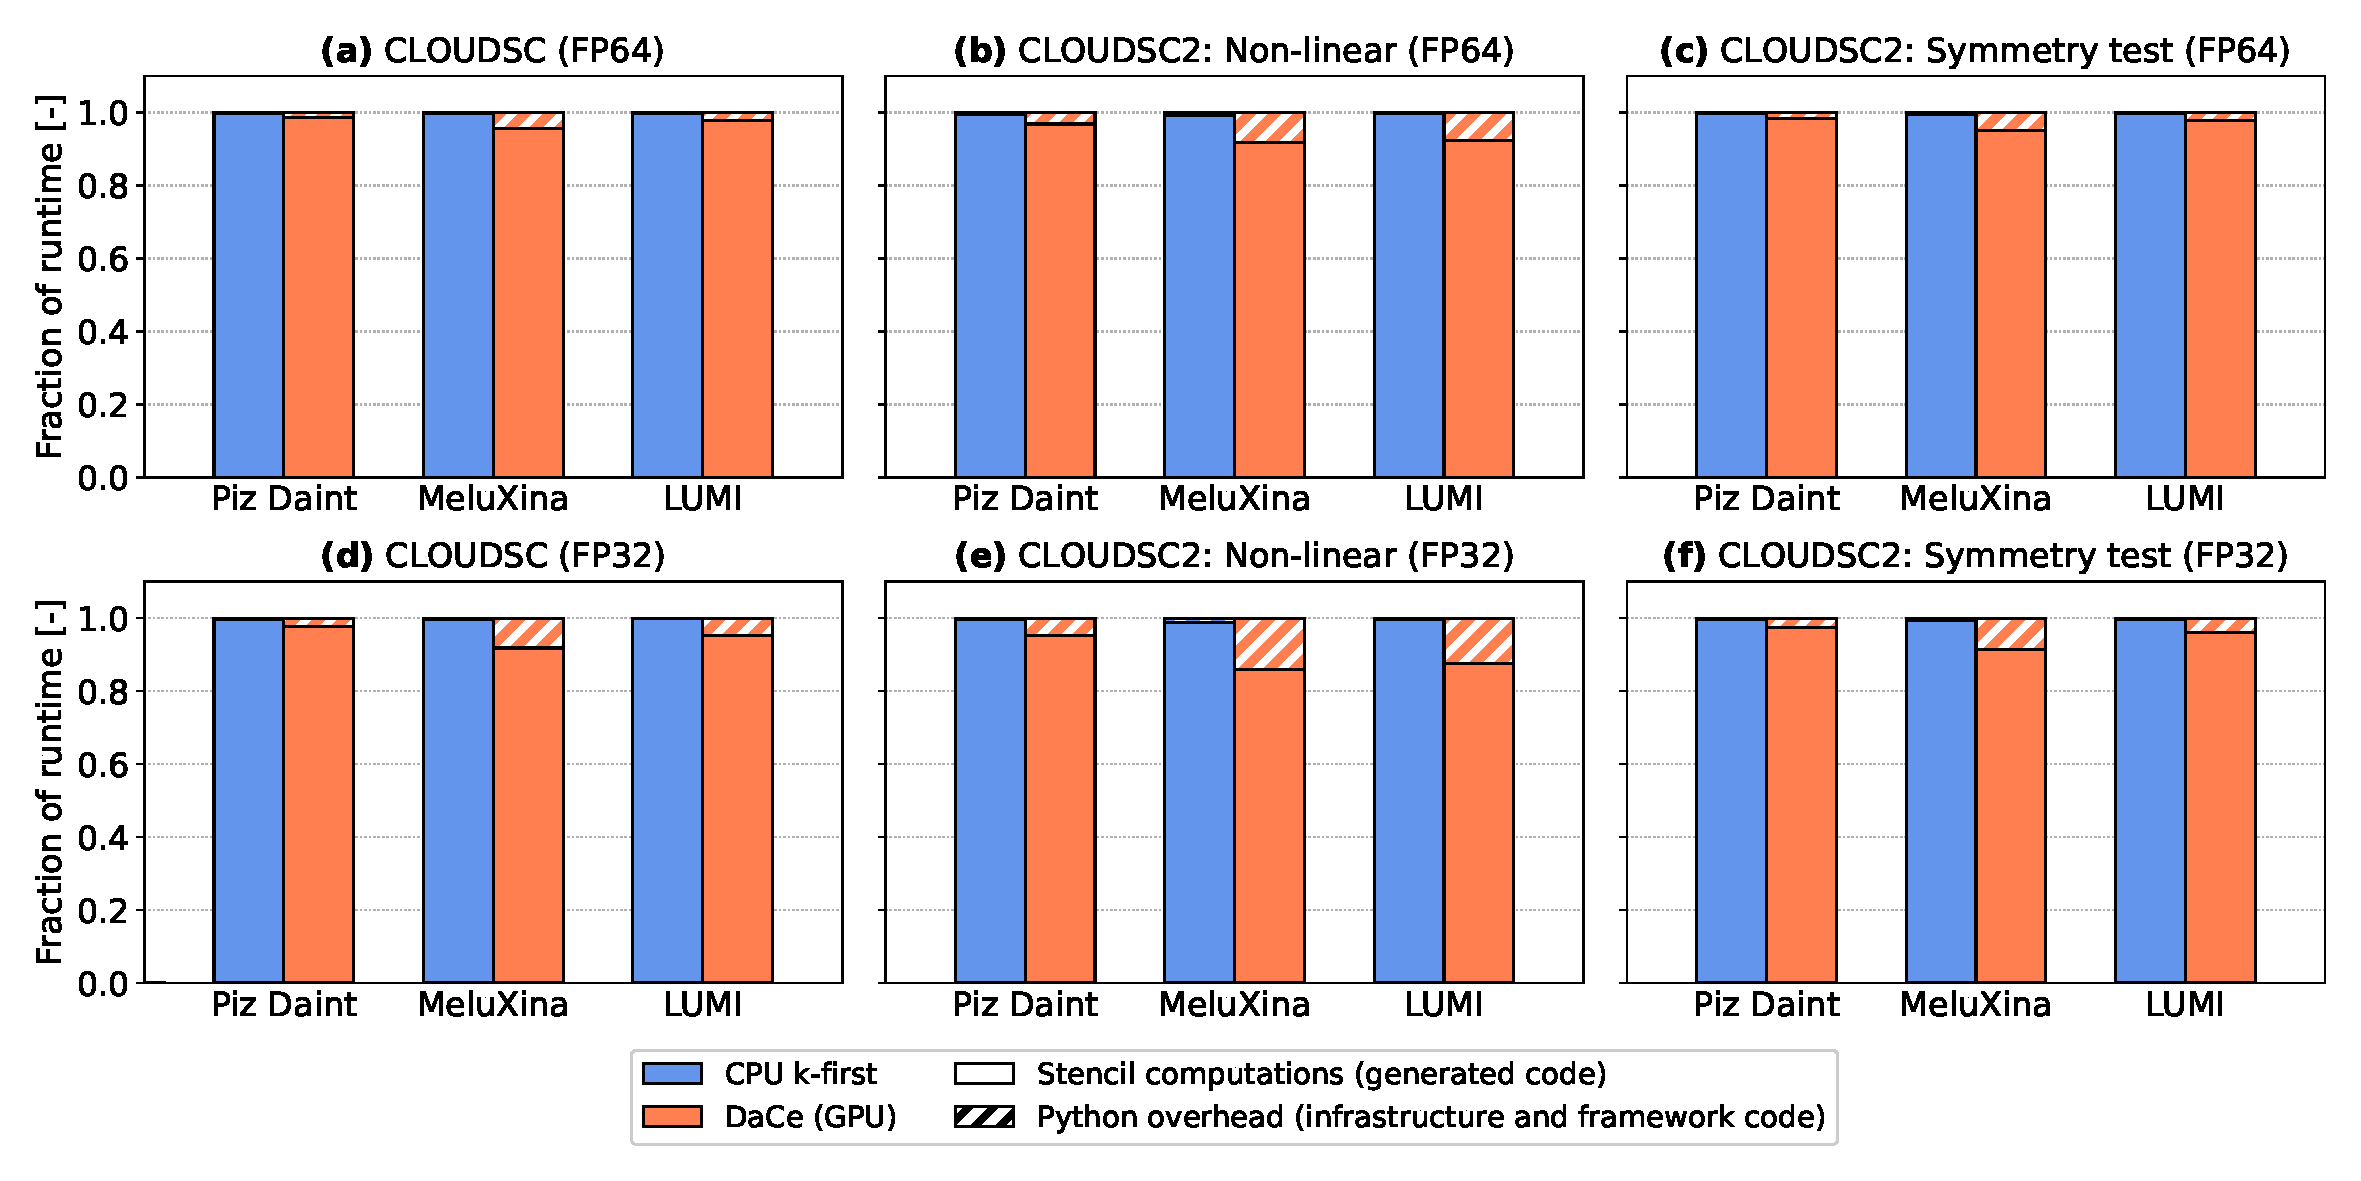
\includegraphics[scale=0.44]{runtime_fraction_1.pdf}
		\caption{For the GT4Py rewrites of CLOUDSC (left column), CLOUDSC2NL (center column) and the symmetry test for CLOUDSC2TL and CLOUDSC2AD (right column), fraction of the total execution time spent within the stencil computations (full bars) and the Python side of the application (hatched bars) on Piz Daint, MeluXina and LUMI. Results are shown for the GridTools C++ CPU backend with k-first data ordering (blue) and the DaCe GPU backend (orange), either using double precision (top row) or single precision (bottom row) floating point arithmetic.}
		\label{fig:runtime-fraction}
	\end{figure}

	To rule out the possibility that the performance gap between the Python DSL and lower-level codes is associated with overhead originating from Python, Fig.\,\ref{fig:runtime-fraction} displays the fraction of runtime spent within the stencil code generated by GT4Py and the high-level Python code of the application (infrastructure and framework code; see Section \ref{section:infrastructure-code}). Across the three supercomputers, the Python overhead decreases as (i) the complexity and length of computations increase, (ii) the peak throughput and bandwidth delivered by the hardware underneath decrease, and (iii) the floating point precision increases. On average, the Python overhead accounts for $5.4\,\%$ of the total runtime on GPU and $0.4\,\%$ on CPU. \DIFaddbegin \DIFadd{Interestingly, if one takes into account only the cases for which a working Fortran CPU implementation is available, even if the GT4Py performance was on par with Fortran, the Python overhead would still amount to less than $0.7\,\%$ of the total execution time on average.
}\DIFaddend 

	Finally, we observe a significant sensitivity of the GPU performance with respect to the thread block size\footnote{In the Fortran code, the thread block size corresponds to the NPROMA.}: for values smaller than 128, performance is degraded across all implementations, with the gap between CUDA/HIP and GT4Py+DaCe being smaller. This shows that some tuning and toolchain optimizations can be performed to improve performance with the DSL approach.

	% ============================================================
	% section 6
	% ============================================================
	\section{Conclusions}
	\label{section:conclusions}

	The CLOUDSC and CLOUDSC2 cloud microphysics schemes of the IFS at ECMWF have served as demonstrators to show the benefits of a high-level domain-specific implementation approach to physical parametrizations. We presented two Python implementations based on the GT4Py framework, in which the scientific code is insulated from hardware-specific aspects. The resulting application provides a productive user interface with enhanced readability and maintainability, and can run efficiently and in a very robust manner across a wide spectrum of compute architectures/systems. The approach can be powerful in the light of the increasingly complex HPC technology landscape, where general-purpose CPUs are increasingly complemented by domain-specific architectures (DSAs) such as GPUs, Tensor Processor Units (TPUs), Field Programmable Gate Arrays (FPGAs), and Application-Specific Integrated Circuits (ASICS). In addition to the CLOUDSC scheme used in the IFS forecast model, we have presented results with the GT4Py rewrites of the nonlinear, tangent-linear and adjoint formulations of CLOUDSC2 used in data assimilation.

	In both CLOUDSC-GT4Py and CLOUDSC2-GT4Py, the stencil kernels are encapsulated within model components sharing a minimal and clear interface. By avoiding any assumption on the host model, the interface aims to provide interoperable and plug-and-play physical packages, which can be transferred more easily between different modeling systems with virtually no performance penalty.

	We carried out a comprehensive study to assess the portability of the Python codes across three major supercomputers, differing in terms of the vendor, the node architecture, the software stack and the compiler suites. We showed that the GPU performance of GT4Py codes are competitive against optimized Fortran OpenACC implementations and perform particularly well when compared to the available codes generated with the Loki source-to-source translation tool. Low-level implementations written either in Fortran for CPUs or CUDA/HIP for GPUs, with additional optimizations that possibly require knowledge about the specific compute patterns, can provide better performance, but are extremely challenging to create and maintain for entire models. The CPU performance of GT4Py is currently suboptimal, but this is an expected result given the focus on GPUs in the DSL development so far and we clearly expect this to improve significantly with upcoming and future GT4Py versions. \DIFaddbegin \DIFadd{Indeed, since the DSL can accommodate any specific low-level optimization, attaining the same performance as native Fortran and CUDA/HIP models is feasible and will be the target of our future efforts.
}\DIFaddend 

	The presented results, based on a representative physical parametrization and considering tangent-linear and adjoint versions, add to the notion that weather and climate model codes can execute significantly faster on GPUs \citep{fuhrer18}, and the number of HPC systems with accelerators is steadily increasing\footnote{In the 62\textsuperscript{nd} edition of the TOP500 list published in November 2023, 186 out of the 500 most powerful supercomputers in the world use graphics accelerator technology (\url{https://www.top500.org/lists/top500/2023/11/highs/}).}. Therefore, we envision that CPUs will be increasingly relegated to tasks that are not time-critical.

	% On the other hand, we recognize that GPU performance are of utter importance in view of a future adoption of GT4Py in an operational context. We believe that the GPU porting of a full-fledged model via a ground-up rewriting using a DSL is not only possible, but also more sustainable and cost-effective than a directive-based approach. Indeed, DSLs enable a separation of concerns between domain scientists and computer experts, so that both can better exploit the respective field of expertise and thus boost their productivity. Notwithstanding, we stress that the development and maintenance of the DSL toolchain with respect to emerging computational patterns and heterogeneous compute platforms is complex and does not come for free. However, provided that the design of the toolchain is driven by a close synergy between domain scientists and computer experts, the advantages for all downstream applications significantly offset the investment in the DSL.

	The current study supports our ongoing efforts and plans to port other physical parametrizations to Python with GT4Py. However, we note that GT4Py has been originally devised to express the computational motifs of dynamical cores based on grid-point methods, so not all patterns found in the parametrizations are natively supported by the DSL. \DIFdelbegin \DIFdel{These cases }\DIFdelend \DIFaddbegin \DIFadd{In this respect, the main limitations of the DSL pertain to data dimensions, single column abstractions, and vertical reductions. These deficiencies }\DIFaddend may be addressed by new features added to GT4Py or by resorting to other Python libraries to generate fast machine code.

	% For instance, absolute indexing and off-center writing are not implemented, so workarounds are needed to update the surface layer from each vertical level and modify two consecutive vertical layers in conjunction.
	% possibly recycling the prototype infrastructure code presented in this manuscript.

	% ============================================================
	%DIF <  acknowledgements
	%DIF >  appendix
	% ============================================================
	\DIFaddbegin \appendix

	\section{\DIFadd{Algorithmic description of the Taylor test and symmetry test for CLOUDSC2}}
	\label{section:appendix}

	\DIFadd{In Section \ref{section:cloudsc2}, we briefly described the aim and functioning of the Taylor test and the symmetry test for CLOUDSC2. Here, we detail the logical steps performed by the two tests with the help of pseudo-codes encapsulated in Algorithms \ref{alg:taylor-test} and \ref{alg:symmetry-test}.
}

	\begin{algorithm}[H]
		\caption{\DIFadd{The Taylor test assessing the formal correctness of the coding implementation of the tangent-linear formulation of CLOUDSC2, denoted as }\textsc{\DIFadd{CLOUDSC2TL}}\DIFadd{. The three-dimensional arrays $\mathbf{x}$ and $\mathbf{y}$ collect the grid point values for all $nin$ input fields and $nout$ output fields of CLOUDSC2, respectively. The corresponding variations are $\delta \mathbf{x}$ and $\delta \mathbf{y}$. The grid consists of $ncol$ columns, each containing $nlev$ vertical levels. Note that compared to its functional counterpart $F' \left[\boldsymbol{x} \right] : \delta \boldsymbol{x} \mapsto \delta \boldsymbol{y}$, }\textsc{\DIFadd{CLOUDSC2TL($\mathbf{x}, \, \delta \mathbf{x}$)}} \DIFadd{returns both $\mathbf{y}$ and $\delta \mathbf{y}$. The coding implementation of the non-linear CLOUDSC2 is indicated as }\textsc{\DIFadd{CLOUDSC2NL}}\DIFadd{.}}
		\label{alg:taylor-test}

		\begin{algorithmic}[1]
			\Function{TotalNorm}{$ncol, \, nlev, \, nout, \, \mathbf{y}, \, \mathbf{y}_j, \, \delta \mathbf{y}_j$} \Comment{$\mathbf{y}, \, \mathbf{y}_j, \, \delta \mathbf{y}_j \in \mathbb{R}^{ncol \times nlev \times nout}$}
			\State \DIFadd{$total\_norm ~ \gets ~ 0$
			}\State \DIFadd{$total\_count ~ \gets ~ 0$
			}\For{l}{1}{nout}
			%DIF > \State $\beta ~ \gets ~ \big| \Call{GetFieldSum}{\delta \mathbf{y}_j \left( :, \, :, \, n \right)} \big|$
				\State \DIFadd{$\beta ~ \gets ~ \big| \sum_{i=1}^{nlev} \sum_{k=1}^{ncol} \delta \mathbf{y}_j \left( i, \, k, \, l \right) \big|$
				}\If{$\beta > 0$}
				%DIF > \State $total\_norm ~ \gets ~ total\_norm + \big| \Call{GetFieldSum}{\mathbf{y}_j \left( :, \, :, \, n \right) - \mathbf{y} \left( :, \, :, \, n \right)} \big| \, / \, \beta$
					\State \DIFadd{$total\_norm ~ \gets ~ total\_norm + \big| \sum_{i=1}^{nlev} \sum_{k=1}^{ncol} \left( \mathbf{y}_j \left( i, \, k, \, l \right) - \mathbf{y} \left( i, \, k, \, l \right) \right) \big| \, / \, \beta$
					}\State \DIFadd{$total\_count ~ \gets ~ total\_count + 1$
				}\EndIf
			\EndFor
			\If{$total\_count > 0$}
				\State \textbf{\DIFadd{return}} \DIFadd{$total\_norm \, / \, total\_count$
			}\Else
				\State \textbf{\DIFadd{return}} \DIFadd{0
			}\EndIf
			\EndFunction

			\Statex

			\Procedure{TaylorTest}{$ncol, \, nlev, \, nin, \, nout, \, \mathbf{x}$} \Comment{$\mathbf{x} \in \mathbb{R}^{ncol \times nlev \times nin}$}

			%DIF > \State $\mathbf{y} ~ \gets ~$ \Call{CLOUDSC2NL}{$\mathbf{x}$}
			\State \DIFadd{$\delta \mathbf{x} ~ \gets ~ 0.01 * \mathbf{x}$
			}\State \DIFadd{$\left( \mathbf{y}, \, \delta \mathbf{y} \right) ~ \gets ~ \Call{CLOUDSC2tl}{\mathbf{x}, \, \delta \mathbf{x}}$ }\Comment{$\mathbf{y}, \, \delta \mathbf{y} \in \mathbb{R}^{ncol \times nlev \times nout}$}
			\State \DIFadd{$norms ~ \gets ~ ()$
			}\State \DIFadd{$jstart ~ \gets ~ 1$
			}\For{j}{1}{10}
			%DIF > \State $\mathbf{x}_j ~ \gets ~ \mathbf{x} + 10^{-j} * \delta \mathbf{x}$
				\State \DIFadd{$\mathbf{y}_j ~ \gets ~ \Call{CLOUDSC2nl}{\mathbf{x} + 10^{-j} * \delta \mathbf{x}}$
				%DIF > \State $\delta \mathbf{y}_j ~ \gets ~ 10^{-j} * \delta \mathbf{y}$
				}\State \DIFadd{$norms ~ \gets ~ norms ~ \cup ~ \left( 1 - \Call{TotalNorm}{ncol, \, nlev, \, nout, \, \mathbf{y}, \, \mathbf{y}_j, \, 10^{-j} * \delta \mathbf{y}} \right)$
				}\If{$jstart = 1 \And norms(j) < 0.5$}
					\State \DIFadd{$jstart \gets j$
				}\EndIf
			\EndFor

			\State{$test ~ \gets ~ -10$}
			\State{$negat ~ \gets ~ \text{True}$}
			\For{j}{jstart}{9}
				\If{$negat \And norms(j+1) \ge norms(j)$}
					\State \DIFadd{$test ~ \gets ~ test + 10$
				}\EndIf
				\State \DIFadd{$negat ~ \gets ~ norms(j+1) < norms(j)$
			}\EndFor
			\If{$test = -10$}
				\State \DIFadd{$test ~ \gets ~ 11$
			}\EndIf
			\If{$\min_{jstart \le j \le 10} \left( {norms(j)} \right) > 10^{-5}$}
				\State \DIFadd{$test ~ \gets ~ test + 7$
			}\EndIf
			\If{$\min_{jstart \le j \le 10} \left( {norms(j)} \right) > 10^{-6}$}
				\State \DIFadd{$test ~ \gets ~ test + 5$
			}\EndIf
			\If{$test \le 5$}
				\State \textbf{\DIFadd{print}} \emph{\DIFadd{"The Taylor test passed."}}
			\Else
				\State \textbf{\DIFadd{print}} \emph{\DIFadd{"The Taylor test failed."}}
			\EndIf
			\EndProcedure
		\end{algorithmic}
	\end{algorithm}

	\begin{algorithm}[t!]
		\caption{\DIFadd{The symmetry test assessing the formal correctness of the coding implementation of the adjoint formulation of CLOUDSC2, denoted as }\textsc{\DIFadd{CLOUDSC2AD}}\DIFadd{. The machine epsilon is indicated as $\varepsilon$; all other symbols have the same meaning as in Algorithm \ref{alg:taylor-test}. Note that compared to its functional counterpart $F^* \left[ F \left( \boldsymbol{x} \right) \right] : \delta \boldsymbol{y} \mapsto \delta \boldsymbol{x}^*$, }\textsc{\DIFadd{CLOUDSC2AD($\mathbf{x}, \, \delta \mathbf{y}$)}} \DIFadd{returns both $\mathbf{y}$ and $\delta \mathbf{x}^*$.}}
		\label{alg:symmetry-test}

		\begin{algorithmic}[1]
			\Function{ColumnWiseInnerProduct}{$ncol, \, nlev, \, ndim, \, \mathbf{a}, \, \mathbf{b}$} \Comment{$\mathbf{a}, \, \mathbf{b} \in \mathbb{R}^{ncol \times nlev \times ndim}$}
			\State \DIFadd{$\boldsymbol{c} ~ \gets ~ \mathbf{0} \in \mathbb{R}^{ncol}$
			}\For{l}{1}{ndim}
				\For{i}{1}{ncol}
					\State \DIFadd{$\boldsymbol{c}(i) ~ \gets ~ \boldsymbol{c}(i) + \sum_{k=1}^{ncol} \mathbf{a} \left( i, \, k, \, l \right) * \mathbf{b} \left( i, \, k, \, l \right)$
				}\EndFor
			\EndFor
			\State \textbf{\DIFadd{return}} \DIFadd{$\boldsymbol{c}$
			}\EndFunction

			\Statex

			\Procedure{SymmetryTest}{$ncol, \, nlev, \, nin, \, nout, \, \mathbf{x}, \varepsilon$} \Comment{$\mathbf{x} \in \mathbb{R}^{ncol \times nlev \times nin}$}

			\State \DIFadd{$\delta \mathbf{x} ~ \gets ~ 0.01 * \mathbf{x}$
			}\State \DIFadd{$\left( \mathbf{y}, \, \delta \mathbf{y} \right) ~ \gets ~ \Call{CLOUDSC2TL}{\mathbf{x}, \, \delta \mathbf{x}}$ }\Comment{$\mathbf{y}, \, \delta \mathbf{y} \in \mathbb{R}^{ncol \times nlev \times nout}$}

			\State \DIFadd{$\left( \mathbf{y}, \, \delta \mathbf{x}^* \right) ~ \gets ~ \Call{CLOUDSC2AD}{\mathbf{x}, \, \delta \mathbf{y}}$ }\Comment{$\mathbf{x}^*, \, \delta \mathbf{x}^* \in \mathbb{R}^{ncol \times nlev \times nin}$}
			\State \DIFadd{$\boldsymbol{c}_{\mathbf{y}} ~ \gets ~ \Call{ColumnWiseInnerProduct}{ncol, \, nlev, \, nout, \, \delta \mathbf{y}, \, \delta \mathbf{y}}$
			}\State \DIFadd{$\boldsymbol{c}_{\mathbf{x}} ~ \gets ~ \Call{ColumnWiseInnerProduct}{ncol, \, nlev, \, nin, \, \delta \mathbf{x}, \, \delta \mathbf{x}^*}$
}

			\State \DIFadd{$success ~ \gets ~ \text{True}$
			}\For{i}{1}{ncol}
				\If{$\boldsymbol{c}_{\mathbf{x}}(i) = 0$}
					\State \DIFadd{$c ~ \gets ~ \left| \boldsymbol{c}_{\mathbf{y}}(i) \right| \, / \, \varepsilon$
				}\Else
					\State \DIFadd{$c ~ \gets ~ \left| \boldsymbol{c}_{\mathbf{y}}(i) - \boldsymbol{c}_{\mathbf{x}}(i) \right| \, / \, \left| \varepsilon * \boldsymbol{c}_{\mathbf{x}}(i) \right|$
				}\EndIf
				\State \DIFadd{$success ~ \gets ~ success \And c < 10^3$
			}\EndFor
			\If{$success$}
				\State \textbf{\DIFadd{print}} \emph{\DIFadd{"The symmetry test passed."}}
			\Else
				\State \textbf{\DIFadd{print}} \emph{\DIFadd{"The symmetry test failed."}}
			\EndIf
			\EndProcedure
		\end{algorithmic}
	\end{algorithm}

	%DIF >  ============================================================
	%DIF >  acknowledgments
	%DIF >  ============================================================
	\DIFaddend \codedataavailability{The source codes for \pyinline{ifs-physics-common} \citep[][\url{https://github.com/stubbiali/ifs-physics-common}]{ifs-physics-common}, CLOUDSC-GT4Py \citep[][\url{https://github.com/stubbiali/gt4py-dwarf-p-cloudsc}]{gt4py-dwarf-p-cloudsc} and CLOUDSC2-GT4Py \citep[][\url{https://github.com/stubbiali/gt4py-dwarf-p-cloudsc2-tl-ad}]{gt4py-dwarf-p-cloudsc2-tl-ad}, as well as the data and scripts to produce all the figures of the paper \citep[][\url{https://github.com/stubbiali/cloudsc-paper}]{gmd-cloudsc-paper}, are available on Github and archived on Zenodo.}

	%% this section is mandatory
	\authorcontribution{SU ported the CLOUDSC and CLOUDSC2 dwarfs to Python using GT4Py and ran all the numerical experiments presented in the paper, under the supervision of CK and HW. SU further contributed to the development of the infrastructure code illustrated in Section \ref{section:infrastructure-code}, under the supervision of CS, LS and TCS. MS made relevant contributions to the Fortran and C reference implementations of the ECMWF microphysics schemes. SU and CK wrote the paper, with feedback from all co-authors.}

	%% this section is mandatory even if you declare that no competing interests are present
	\competinginterests{The authors declare that they have no conflict of interest.}

	%% optional section
	%\disclaimer{TEXT}

	\begin{acknowledgements}
		\DIFaddbegin \DIFadd{We would like to thank three anonymous referees for carefully reviewing the manuscript and providing many constructive comments. }\DIFaddend This study was conducted as part of the Platform for Advanced Scientific Computing (PASC) funded project KILOS (``Kilometer-scale non-hydrostatic global weather forecasting with IFS-FVM''), which also provided us with computing resources on the Piz Daint supercomputer at CSCS. \DIFaddbegin \DIFadd{CK has received funding from the ESiWACE3 project funded by the European High Performance Computing Joint Undertaking (EuroHPC JU) and the European Union (EU) under grant agreement No 101093054. }\DIFaddend We acknowledge EuroHPC JU for awarding the project ID 200177 access to the MeluXina supercomputer at LuxConnect and the project ID 465000527 access to the LUMI system at CSC, and thank Thomas Geenen and Nils Wedi from Destination Earth for their help. We are grateful to Michael Lange and Balthasar Reuter for discussions and support regarding IFS codes.
	\end{acknowledgements}

	% ============================================================
	% bibliography
	% ============================================================
	\DIFdelbegin %DIFDELCMD < \bibliography{references_v0}
%DIFDELCMD < %%%
\DIFdelend \DIFaddbegin \bibliography{references_v1}
\DIFaddend 

% ============================================================
% end document
% ============================================================
\end{document}

% ============================================================
% more information and advice
% ============================================================
%% FIGURES

%% When figures and tables are placed at the end of the MS (article in one-column style), please add \clearpage
%% between bibliography and first table and/or figure as well as between each table and/or figure.

% The figure files should be labelled correctly with Arabic numerals (e.g. fig01.jpg, fig02.png).


%% ONE-COLUMN FIGURES

%%f
%\begin{figure}[t]
%\includegraphics[width=8.3cm]{FILE NAME}
%\caption{TEXT}
%\end{figure}
%
%%% TWO-COLUMN FIGURES
%
%%f
%\begin{figure*}[t]
%\includegraphics[width=12cm]{FILE NAME}
%\caption{TEXT}
%\end{figure*}
%
%
%%% TABLES
%%%
%%% The different columns must be seperated with a & command and should
%%% end with \\ to identify the column brake.
%
%%% ONE-COLUMN TABLE
%
%%t
%\begin{table}[t]
%\caption{TEXT}
%\begin{tabular}{column = lcr}
%\tophline
%
%\middlehline
%
%\bottomhline
%\end{tabular}
%\belowtable{} % Table Footnotes
%\end{table}
%
%%% TWO-COLUMN TABLE
%
%%t
%\begin{table*}[t]
%\caption{TEXT}
%\begin{tabular}{column = lcr}
%\tophline
%
%\middlehline
%
%\bottomhline
%\end{tabular}
%\belowtable{} % Table Footnotes
%\end{table*}
%
%%% LANDSCAPE TABLE
%
%%t
%\begin{sidewaystable*}[t]
%\caption{TEXT}
%\begin{tabular}{column = lcr}
%\tophline
%
%\middlehline
%
%\bottomhline
%\end{tabular}
%\belowtable{} % Table Footnotes
%\end{sidewaystable*}
%
%
%%% MATHEMATICAL EXPRESSIONS
%
%%% All papers typeset by Copernicus Publications follow the math typesetting regulations
%%% given by the IUPAC Green Book (IUPAC: Quantities, Units and Symbols in Physical Chemistry,
%%% 2nd Edn., Blackwell Science, available at: http://old.iupac.org/publications/books/gbook/green_book_2ed.pdf, 1993).
%%%
%%% Physical quantities/variables are typeset in italic font (t for time, T for Temperature)
%%% Indices which are not defined are typeset in italic font (x, y, z, a, b, c)
%%% Items/objects which are defined are typeset in roman font (Car A, Car B)
%%% Descriptions/specifications which are defined by itself are typeset in roman font (abs, rel, ref, tot, net, ice)
%%% Abbreviations from 2 letters are typeset in roman font (RH, LAI)
%%% Vectors are identified in bold italic font using \vec{x}
%%% Matrices are identified in bold roman font
%%% Multiplication signs are typeset using the LaTeX commands \times (for vector products, grids, and exponential notations) or \cdot
%%% The character * should not be applied as mutliplication sign
%
%
%%% EQUATIONS
%
%%% Single-row equation
%
%\begin{equation}
%
%\end{equation}
%
%%% Multiline equation
%
%\begin{align}
%& 3 + 5 = 8\\
%& 3 + 5 = 8\\
%& 3 + 5 = 8
%\end{align}
%
%
%%% MATRICES
%
%\begin{matrix}
%x & y & z\\
%x & y & z\\
%x & y & z\\
%\end{matrix}
%
%
%%% ALGORITHM
%
%\begin{algorithm}
%\caption{...}
%\label{a1}
%\begin{algorithmic}
%...
%\end{algorithmic}
%\end{algorithm}
%
%
%%% CHEMICAL FORMULAS AND REACTIONS
%
%%% For formulas embedded in the text, please use \chem{}
%
%%% The reaction environment creates labels including the letter R, i.e. (R1), (R2), etc.
%
%\begin{reaction}
%%% \rightarrow should be used for normal (one-way) chemical reactions
%%% \rightleftharpoons should be used for equilibria
%%% \leftrightarrow should be used for resonance structures
%\end{reaction}
%
%
%%% PHYSICAL UNITS
%%%
%%% Please use \unit{} and apply the exponential notation
